\documentclass[a4paper,11pt]{article}

\usepackage[utf8]{inputenc}
\usepackage[T1]{fontenc}
\usepackage[english]{babel}
\usepackage[a4paper,top=2.4cm,bottom=2.4cm,left=2.4cm,right=2.4cm]{geometry}
\usepackage{mathptmx}
\usepackage{microtype}
\usepackage{setspace}
\usepackage{amsmath,amssymb,amsfonts,mathtools}
\usepackage{graphicx}
\usepackage{subcaption}
\usepackage{booktabs}
\usepackage{tabularx}
\usepackage{array}
\usepackage{siunitx}
\usepackage{enumitem}
\usepackage{algorithm}
\usepackage{algpseudocode}
\usepackage{csquotes}
\usepackage{xcolor}
\usepackage{cite}
\usepackage{hyperref}
\usepackage{authblk}

\onehalfspacing
\graphicspath{{figures/}}
\setlength{\emergencystretch}{3em}

\hypersetup{hidelinks}

\sisetup{
    mode=match,
    propagate-math-font=true,
    reset-math-version=false,
    reset-text-family=false,
    reset-text-series=false,
    reset-text-shape=false,
    text-family-to-math=true,
    text-series-to-math=true,
    round-mode=places,
    round-precision=2
}

\newcolumntype{Y}{>{\raggedright\arraybackslash}X}
\title{Path Planning and Obstacle Avoidance Real-Time Collision Evasion: A Deterministic Real-Time Local Replanning Method for Autonomous UAV Power-Line Inspection}
\author[1,2]{Pablo De Porcellinis}
\author[1]{Xabier Olaz}
\author[1,3]{Jes\'us Villadangos}
\affil[1]{Mathematical Engineering and Computer Science Department, Public University of Navarre, Spain}
\affil[2]{FuVeX Civil SL, Spain}
\affil[3]{Institute of Smart Cities, Public University of Navarre, Spain}
\date{}

\begin{document}

\maketitle

\begin{abstract}
Autonomous UAV obstacle avoidance is not new, but most existing algorithms focus on collision-free flight, geometric efficiency, or dynamic feasibility. Much less work addresses the European regulatory logic that an autonomous route should avoid exposing uninvolved people and other protected ground parties to unnecessary overflight risk. This paper presents Path Planning and Obstacle Avoidance Real-Time Collision Evasion, a deterministic real-time local replanning method for waypoint-preserving obstacle avoidance in autonomous power-line inspection missions. The method is implemented and evaluated inside Pipeline A, the validated \texttt{SIMULATION} workflow of the Deep-AeroTwin project, where it operates together with a waypoint-driven flight controller, a YOLO-based perception front-end, monocular obstacle geopositioning, and zero-trust audit logging. In the current implementation, civilian-like detections and nearby entities are converted into protected local no-fly regions that trigger conservative detours instead of nominal overflight. Based on the literature reviewed for 2024--2026, we are not aware of a published method that combines this EASA-motivated no-overflight objective with deterministic online local replanning and autonomous power-line inspection integration in the same way.

Controlled E2E experiments over ten or more runs per scenario show that the method changes the vehicle trajectory only when detections are present and the avoidance module is enabled; under that condition, mission path length increases from $1455.5 \pm 0.2$ to $1463.8 \pm 1.4$ meters (\SI{0.57}{\percent}) and mission time from $205.0 \pm 0.0$ to $207.1 \pm 0.3$ seconds (\SI{1.0}{\percent}), with every mission completed. In the audited zero-trust case study, executed against a live Unreal Engine 5.7 digital twin with a sixteen-rider cycling peloton crossing the inspection corridor at a realistic \SI{23}{\kilo\meter\per\hour}, the method triggers at \SI{35.11}{\meter} on fifteen concurrently published \texttt{biker} tracks, records the sixteen planner obstacle identities in the route event, completes the maneuver in \SI{19.48}{\second} with a local detour of only \SI{3.42}{\meter} over the straight segment, and maintains a minimum time-synchronized separation of \SI{34.27}{\meter} from the tracked obstacles, i.e. \SI{22.27}{\meter} above the configured \SI{12}{\meter} safety radius. These results support the method as a reproducible, low-overhead, and auditable local replanning method that operationalizes part of the European ground-risk logic at the online controller level, while Pipeline A provides the integration and validation environment used to characterize its behavior.
\end{abstract}

\noindent\textbf{Keywords:} local replanning, UAV inspection, obstacle avoidance, ground risk, uninvolved people, SORA, A* replanning, safety-critical navigation

\section{Introduction}

Unmanned Aerial Vehicles (UAVs) are becoming a practical tool for infrastructure inspection, surveillance, and monitoring, with growing impact across agriculture, critical infrastructure, and other industrial environments \cite{imran2025environmental,marut2024surveillance}. Power-line inspection is one of the most relevant of these use cases because it combines long-range navigation, repeated geometric structures, tight mission corridors, and the need to react to unexpected obstacles without compromising the inspection objective.

From a planning standpoint, this scenario is difficult because the vehicle must preserve a global mission structure while responding online to local conflicts. Purely global planners are efficient when the environment is static and fully known, but they become brittle under late obstacle appearance or perception uncertainty \cite{debnath2024review,meng2025advances}. On the other hand, fully learned end-to-end policies are harder to audit in safety-critical aeronautical contexts, where traceability and bounded behavior remain important design properties \cite{EASA_AI_Roadmap_2.0}.

The regulatory dimension makes the problem even sharper. Under the European Union UAS regulatory framework, the operational core is defined by Commission Implementing Regulation (EU) 2019/947 on the rules and procedures for the operation of unmanned aircraft and Commission Delegated Regulation (EU) 2019/945 on unmanned aircraft systems, while EASA AMC/GM material now incorporates the JARUS SORA 2.5 package for the `specific' category \cite{EU2019_947,EU2019_945,JARUS_SORA_2_5_2024,EASA_AMC_GM_SORA25_2025}. Within this framework, the acceptability of a route is not only a matter of geometric collision avoidance but also of limiting exposure of uninvolved people and sensitive ground areas. This means that an autonomous planner should not merely ask whether the UAV \emph{can} fly over a location, but whether it \emph{should} do so in a risk-aware operational sense. Existing literature has already started to encode this concern through urban risk maps, third-party-risk models, SORA-aware cost functions, and target-level-of-safety constraints \cite{primatesta2019riskaware,primatesta2020groundrisk,pang2022integrated,tang2023thirdparty,zhang2023groundrisk,heinze2023sora,brassel2025riskaware}. However, most of these works remain strategic route optimizers or city-scale risk planners rather than controller-level local replanners for infrastructure inspection missions already in progress.

Two regulatory details are especially relevant for interpreting the contribution correctly. First, even outside the `specific' category, the European notion of an uninvolved person makes separation a dynamic operational constraint rather than a purely geometric one: as altitude, corridor geometry, and local context change, the practical exclusion region around people on the ground also changes. Second, under SORA 2.5 in the `specific' category, mitigations such as ground observation explicitly reward the capability to detect uninvolved people and avoid overflight in operation \cite{JARUS_SORA_2_5_2024,EASA_AMC_GM_SORA25_2025}. The present paper does not claim to encode the full legal tables of open-category separation or the full SORA mitigation calculus inside the planner. Instead, it implements the narrower controller-level step that those regulatory mechanisms motivate: live civilian-like detections are converted into temporary protected regions that the UAV should avoid crossing.

This paper focuses on Path Planning and Obstacle Avoidance Real-Time Collision Evasion as the main scientific contribution. The method is a local conflict-resolution system designed for the validated \texttt{SIMULATION} workflow available in the Deep-AeroTwin repository, where a mission file, a flight controller, an onboard-like perception stack, and a local planner operate together in closed loop. Its role is simple but operationally important: whenever an obstacle enters a conservative reaction horizon, the method temporarily inhibits nominal navigation, computes a bounded local path toward the current mission waypoint, and returns control to the original route as soon as the local conflict disappears. The novelty is therefore not obstacle avoidance in isolation. The novelty is to operationalize a regulatory-aware no-overflight logic for uninvolved third parties and nearby protected entities inside a deterministic, auditable, online local replanner. The claim of the paper is correspondingly narrow: the method is advanced as a state-of-the-art contribution in this specific EASA-relevant niche, not as a claim to supersede the broader literature on generic UAV avoidance or strategic risk-aware routing.

The main contributions of the paper are the following.
\begin{itemize}[leftmargin=1.3em]
    \item The definition of Path Planning and Obstacle Avoidance Real-Time Collision Evasion as a deterministic, waypoint-preserving local replanning method for real-time UAV obstacle avoidance in power-line inspection missions, explicitly motivated by European ground-risk and no-overflight concerns.
    \item A formal and reproducible description of how the method is integrated with perception, mission execution, and audit logging inside the validated Pipeline A environment.
    \item An evidence-driven evaluation of the method grounded on repository artifacts, including controlled ablation logs and an audited case study with figures, tables, and derived metrics.
\end{itemize}

\section{State of the Art, Ground-Risk Regulation, and Research Gap}

Vision-based UAV navigation has been widely studied as a perception-driven alternative to map-only planning, with applications ranging from localization to obstacle detection and local trajectory generation \cite{arafat2023vision,huang2025investigation}. General reviews consistently distinguish between global path planning, which assumes a sufficiently known environment, and local path planning, which reacts to obstacles while the vehicle is already moving \cite{debnath2024review,meng2025advances}. More specifically, recent surveys in 2025 and 2026 confirm that the dominant design goals remain collision avoidance, dynamic feasibility, and computational efficiency, while explicit treatment of third-party ground exposure is still comparatively rare in runtime planning \cite{merei2025survey,nafees2026review}. The proposed method is explicitly positioned in the online local-replanning class.

However, there is a second distinction that matters for this paper and that was often implicit in earlier project notes: much of the academic literature is still evaluated under what may be called a \emph{toy-problem bias}. In those formulations, the navigation problem is simplified enough to validate a planner mathematically, but the same simplifications weaken direct transfer to operational infrastructure inspection. Three simplifications are especially consequential here.
\begin{itemize}[leftmargin=1.3em]
    \item \textbf{Obstacle homogeneity.} Obstacles are often represented as interchangeable geometric primitives or generic occupied cells. In inspection practice, this is not operationally neutral: a tower, a cow, and an uninvolved person may all occupy space, but they do not carry the same legal or operational meaning.
    \item \textbf{Binary safety.} Many planners implicitly treat a mission as successful as long as physical collision is avoided. For European civil UAS operations, that criterion is too weak because a near overflight of uninvolved people may already be operationally unacceptable even when no impact occurs \cite{EU2019_947,JARUS_SORA_2_5_2024,EASA_AMC_GM_SORA25_2025}.
    \item \textbf{Free-space permissiveness.} Conventional local planning usually assumes that any geometrically free air volume is candidate flight space. In European operations, parts of that free volume may still be undesirable or prohibited once uninvolved people, sensitive ground areas, or risk buffers are considered.
\end{itemize}
This is why the present paper does not frame the problem as generic collision avoidance alone. It frames it as online mission execution under geometric and regulatory pressure at the same time.

For power-line inspection, the local planning problem is more operational than academic. The vehicle must continue progressing through a mission corridor while structures, animals, vehicles, or uninvolved people may appear in the neighborhood of the route. Power-line inspection has therefore developed its own system literature, from UAV-image approaches for corridor measurement and obstacle localization \cite{zhang2017powerline} to line detection in cluttered scenes \cite{zhang2019powerlines}, LiDAR-supported automatic inspection \cite{guan2021uavlidar}, dual-view stereovision for reconstruction and clearance estimation \cite{zhou2022dualview}, and dedicated reviews of UAV-enabled power-line inspection \cite{mendu2025state}. On the perception side, Bellou \emph{et al.} report YOLOv8-based aerial inspection for towers, conductors, and insulators \cite{bellou2024aerial}, while Faisal \emph{et al.} synthesize more than 70 studies and identify persistent gaps in multimodal fusion and deployment realism \cite{faisal2025deep}. On the planning side, Huang \emph{et al.} propose a hybrid RRT*+DWA method for dynamic obstacle avoidance in UAV-based power inspection \cite{huang2025hybrid}. These works are highly relevant, but their central objective is still efficient and safe inspection autonomy, not explicit no-overflight treatment of uninvolved people under European operational logic.

That regulatory logic matters because, under the European Union UAS framework defined by Regulations (EU) 2019/947 and 2019/945 and operationalized through AMC/GM plus SORA 2.5, route acceptability is not only about avoiding collision with obstacles but also about limiting exposure of uninvolved people and other protected ground parties \cite{EU2019_947,EU2019_945,JARUS_SORA_2_5_2024,EASA_AMC_GM_SORA25_2025}. A separate strand of literature already addresses this concern directly. Primatesta \emph{et al.} propose a risk-aware urban path-planning strategy with off-line and on-line phases driven by risk maps \cite{primatesta2019riskaware}, and later formalize the construction of ground-risk maps for urban UAV operations \cite{primatesta2020groundrisk}. Pang \emph{et al.} optimize routes by integrating third-party risks into a metropolitan cost model \cite{pang2022integrated}. Tang \emph{et al.} explicitly model obstacle risk, fatality risk, and property loss risk in a Min-cost A* framework \cite{tang2023thirdparty}. Pilko \emph{et al.} and Zhu \emph{et al.} extend the discussion toward spatiotemporal and grid-based ground-risk mapping \cite{pilko2023spatiotemporal,zhang2023groundrisk}. Heinze and Uijt de Haag, and more recently Bra{\ss}el \emph{et al.}, push this line closer to current European operations by encoding SORA and TLS concepts into route optimization \cite{heinze2023sora,brassel2025riskaware}. Complementarily, Du \emph{et al.} review safety-risk modeling for civil UAS operations and show how strongly current safety research is centered on assessment and authorization-oriented risk modeling \cite{du2024safetyrisk}.

The regulatory interpretation also differs depending on the operational category, and this nuance is important for interpreting the method correctly. In the \emph{open} category, the concept of \emph{uninvolved person} already implies that route geometry cannot be judged independently from who may be under the aircraft and under what conditions. In the \emph{specific} category, SORA 2.5 shifts the discussion toward operational volume, ground-risk buffers, and mitigations such as ground observation, all of which make in-operation awareness of people on the ground strategically useful \cite{EU2019_947,JARUS_SORA_2_5_2024,EASA_AMC_GM_SORA25_2025}. The present method does not implement the full legal machinery of either category. What it does implement is the controller-level behavior that both categories motivate: when live perception suggests that the current local corridor should not be overflown, the UAV performs a temporary local bypass instead of persisting on the nominal line.

The most recent SOTA from 2024 to 2026 further sharpens the distinction between strategic risk planning and controller-level reaction. ElSayed and Mohamed (2024) integrate digital-twin airspace discretization with trajectory optimization under legal and operational constraints \cite{elsayed2024digitaltwin}. Pang \emph{et al.} (2024) model dynamic ground-risk uncertainty for safe drone delivery through stochastic route optimization \cite{pang2024stochastic}. Zhou \emph{et al.} (2025) propose a risk-based path-planning scheme for complex air--ground environments \cite{zhou2025riskbased}, while Riedel (2025) reviews detect-and-avoid standards and shows how strongly recent compliance discussions are still centered on air-risk, separation, and certification interfaces rather than overflight of uninvolved people on the ground \cite{riedel2025daa}. Checker \emph{et al.} (2025) review mission planning from a regulatory perspective, but at the swarm and mission-allocation level \cite{checker2025regulatory}. In 2026, Zhu \emph{et al.} move toward adaptive urban airspace allocation under uncertainty \cite{zhu2026adaptive}, and Nafees \emph{et al.} summarize the broader planning landscape while still highlighting real-time adaptation and constraint integration as open challenges \cite{nafees2026review}. Collectively, these works show that the field is advancing quickly, but the newest contributions still concentrate on strategic routing, digital twins, logistics airspace, or standards alignment more than on deterministic local replanning for inspection missions already underway.

This prior art is real and important, so the contribution of the proposed method must be framed carefully. The method is not the first UAV system to consider people on the ground, nor the first planner to use risk-aware costs. The narrower and more defensible claim is operational: existing inspection planners usually optimize geometric avoidance without an explicit uninvolved-people objective, whereas existing ground-risk and SORA-aware planners usually operate at strategic, route-design, or city-map scale. What remains weakly addressed is the controller-level problem of how an autonomous inspection UAV should react \emph{online}, during a running mission, when live detections suggest that the nominal corridor would overfly or closely pass above a civilian-like entity. The proposed method addresses exactly that intersection by converting nearby detections into protected local no-fly regions, preserving the active mission waypoint as the anchor of the maneuver, and exposing the resulting decisions through the same telemetry, API, and audit chain used by Pipeline A. To the best of our knowledge after reviewing the 2024--2026 literature, this makes the method a state-of-the-art contribution in the narrow niche of EASA-motivated, controller-level, inspection-integrated local replanning for uninvolved-people-aware UAV operation.

\begin{table}[t]
    \centering
    \caption{Representative 2024--2026 comparison between recent SOTA strands and the proposed method.}
    \label{tab:sota_positioning}
    \footnotesize
    \begin{tabularx}{\linewidth}{@{}Y Y Y@{}}
        \toprule
        \textbf{Representative work} & \textbf{What it already solves} & \textbf{Remaining gap relative to the proposed method} \\
        \midrule
        ElSayed and Mohamed (2024); Zhu \emph{et al.} (2026) \cite{elsayed2024digitaltwin,zhu2026adaptive} & Digital-twin airspace structuring and adaptive urban allocation under legal, operational, and uncertainty constraints & They operate mainly at city-airspace and logistics scale, not at the live local-replanning layer of an inspection UAV reacting to a detected civilian-like obstacle \\
        Pang \emph{et al.} (2024); Zhou \emph{et al.} (2025); Bra{\ss}el \emph{et al.} (2025) \cite{pang2024stochastic,zhou2025riskbased,brassel2025riskaware} & Strong third-party-risk, ground-risk, and TLS-aware optimization of routes & Their main contribution is strategic or pre-flight route optimization rather than short-horizon mission-preserving replanning inside an active inspection controller \\
        Riedel (2025); Checker \emph{et al.} (2025) \cite{riedel2025daa,checker2025regulatory} & Up-to-date synthesis of detect-and-avoid standards and regulatory mission-planning constraints & They clarify standards and regulatory context, but they do not provide a controller-level method for avoiding overflight of uninvolved people from live detections \\
        Bellou \emph{et al.} (2024); Huang \emph{et al.} (2025) \cite{bellou2024aerial,huang2025hybrid} & Inspection-specific perception and dynamic obstacle avoidance for power-line operations & They improve inspection autonomy, but not around an explicit European no-overflight / ground-risk objective for uninvolved third parties \\
        \textbf{This paper} & \textbf{Deterministic waypoint-preserving local replanning triggered by live detections inside an autonomous inspection mission} & \textbf{Brings protected-ground logic, controller integration, and auditability together in Pipeline A rather than treating them as separate planning, perception, and compliance layers} \\
        \bottomrule
    \end{tabularx}
\end{table}

Within the local-planning literature, deterministic graph search remains appealing for safety-critical systems because completeness and failure modes are easier to inspect than in stochastic black-box policies. A* provides precisely that balance between computational simplicity and interpretable behavior \cite{hart1968formal}. The proposed method builds on that property and combines it with a YOLO-based perception front-end \cite{ultralytics_yolo} and monocular obstacle geopositioning inspired by the real-time method proposed in \cite{alaez2023real}.

\section{System Integration in Pipeline A}

The proposed method is evaluated inside Pipeline A, the validated \texttt{SIMULATION} workflow in the repository. Figure~\ref{fig:pipeline_architecture} summarizes the runtime architecture: the mission file, visual source, and MAVLink telemetry enter the Brain; the vision module publishes georeferenced obstacle tracks; the PORCE planner returns a bounded local route; and the same execution state is exposed through both the runtime API and zero-trust audit artifacts.

\begin{figure}[t]
    \centering
    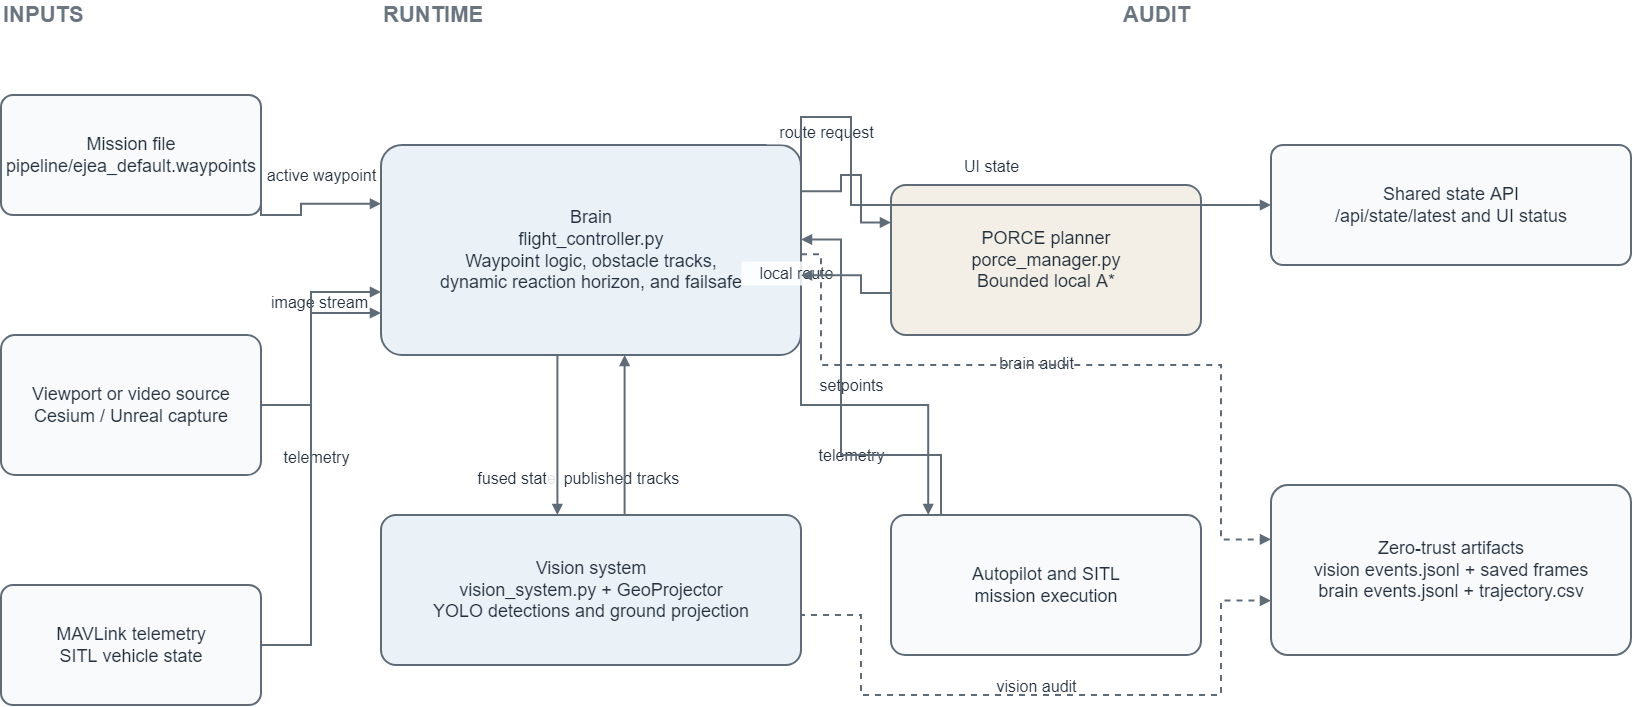
\includegraphics[width=\linewidth]{pipeline_a_architecture.png}
    \caption{Pipeline A runtime architecture used to evaluate the proposed method. Solid arrows indicate runtime data and control flow, while dashed arrows indicate audit and observability outputs.}
    \label{fig:pipeline_architecture}
\end{figure}

The software roles are the following.
\begin{itemize}[leftmargin=1.3em]
    \item \textbf{Mission input:} the file \texttt{pipeline/ejea\_default.waypoints} contains the nominal inspection route.
    \item \textbf{Brain:} \texttt{flight\_controller.py} executes the control loop, manages waypoints, handles failsafe logic, and calls the replanning module whenever local replanning is necessary.
    \item \textbf{Perception:} \texttt{vision\_system.py} runs a YOLO-based detector and projects detections into geographic coordinates using onboard state and monocular geometry \cite{alaez2023real}.
    \item \textbf{Planner:} \texttt{porce\_manager.py} implements the bounded A* local planner used to generate short-range evasion paths.
    \item \textbf{Audit and visualization:} \texttt{trajectory.csv}, \texttt{events.jsonl}, and the visualization endpoint expose the evolution of the mission for analysis and debugging.
\end{itemize}

\subsection{Runtime Integration with Pipeline A}

The integration of the proposed method into Pipeline A is a closed-loop runtime contract rather than a loose module coupling. First, the mission is loaded from a QGroundControl waypoint file and the Brain receives vehicle telemetry from SITL through MAVLink. Second, the perception subsystem queries the latest fused vehicle state and publishes detected obstacles to the Brain through \texttt{POST /api/obstacles}. The Brain then normalizes obstacle classes, enforces source filtering and token validation, maintains obstacle tracks with time-to-live logic, and rebuilds the active obstacle list used for decision making.

In the current implementation, human-adjacent detections are already given a dedicated operational treatment. The labels \texttt{person}, \texttt{bicycle}, and \texttt{biker} are canonicalized into the same dynamic obstacle family, while \texttt{tower} and \texttt{cow} are treated as static classes for tracking and association purposes. This is not yet a full legal ontology of uninvolved people, but it is the concrete mechanism by which civilian-like detections become protected local regions that the method must avoid rather than overfly.

Third, the method is only evaluated when the autonomous mission is active, fresh obstacle evidence exists, and the nearest obstacle crosses a speed-adaptive reaction horizon. Before invoking the planner, the Brain forms a bounded obstacle subset for local replanning: in the validated configuration, only obstacles inside \SI{55}{\meter} and up to 16 tracks are passed to the planner. This keeps the replanning problem short-range and explicitly tied to the current mission waypoint instead of allowing corridor-wide route redefinition.

Fourth, the Brain calls \texttt{PorcePlanner.plan\_route(start, goal, obstacles)}, where the start is the current telemetry position and the goal is the current mission waypoint. The planner inflates each obstacle by the configured safety radius, discretizes the neighborhood into a local \(81 \times 81\) occupancy grid with \SI{6}{\meter} cells, runs bounded A*, and converts the resulting grid path back into geographic sub-points. If a valid route is found, the Brain stores it as the active evasion path; if not, the integration layer escalates through hold, lateral replan, and terminal failsafe actions.

Finally, the method outputs are consumed by the rest of Pipeline A through two channels. On the control side, the Brain sends each local replanning sub-point to the autopilot as MAVLink position-target commands until the evasion route is completed, at which point nominal waypoint following resumes automatically. On the observability side, the same state is exposed through the UI endpoint together with evasion metadata, planner parameters, tracked obstacles, and audit counters, so visualization tools, Unreal consumers, and zero-trust logs all observe the same decision chain. This shared contract is what makes the method not just a planner in isolation, but a reproducible system integrated into a full autonomous inspection pipeline.

Table~\ref{tab:config} summarizes the main runtime parameters used to evaluate the method inside Pipeline A. These values come from the validated simulation defaults already present in the repository.

\begin{table}[t]
    \centering
    \caption{Main configuration values of the validation environment and the proposed method used throughout the paper.}
    \label{tab:config}
    \small
    \begin{tabularx}{\linewidth}{@{}l l Y@{}}
        \toprule
        \textbf{Parameter} & \textbf{Value} & \textbf{Role} \\
        \midrule
        Mission file & 12 waypoints & Nominal inspection route with takeoff and landing phases \\
        Control-loop period & \SI{0.10}{\second} & Brain update period \\
        Cruise speed & \SI{8}{\meter\per\second} & Nominal horizontal mission speed \\
        Grid cell size & \SI{6}{\meter} & Local A* discretization step \\
        Grid radius & 40 cells & Local search radius, i.e. an \(81 \times 81\) occupancy grid \\
        Obstacle safety radius & \SI{12}{\meter} & Hard inflation radius around each obstacle \\
        Base reaction distance & \SI{45}{\meter} & Minimum horizon for replanning activation \\
        Reaction gain & \SI{2.0}{\second} & Speed-dependent enlargement of reaction horizon \\
        Reaction range & \SIrange{45}{80}{\meter} & Clamped reaction distance interval \\
        Route-point tolerance & \SI{3}{\meter} & Distance to accept a local replanning sub-goal as reached \\
        Failsafe threshold & \SI{22}{\meter} & Distance used for hold/lateral replan escalation \\
        Failsafe hold & \SI{2.5}{\second} & Temporary hold action when replanning fails \\
        \bottomrule
    \end{tabularx}
\end{table}

\section{Method Description}

The controller-level logic that constitutes the scientific core of the proposed method is shown in Figure~\ref{fig:porce_method_flow}. The method receives the active waypoint, fresh perception outputs, and current telemetry; canonicalizes human-adjacent detections into protected local regions; evaluates whether the nearest obstacle enters the dynamic reaction horizon; and either preserves nominal mission following or activates a bounded A* local bypass. Importantly, the same decision chain also defines the fallback behavior and the audit outputs, so the proposal is not just a path planner but a complete online conflict-resolution policy.

\begin{figure}[t]
    \centering
    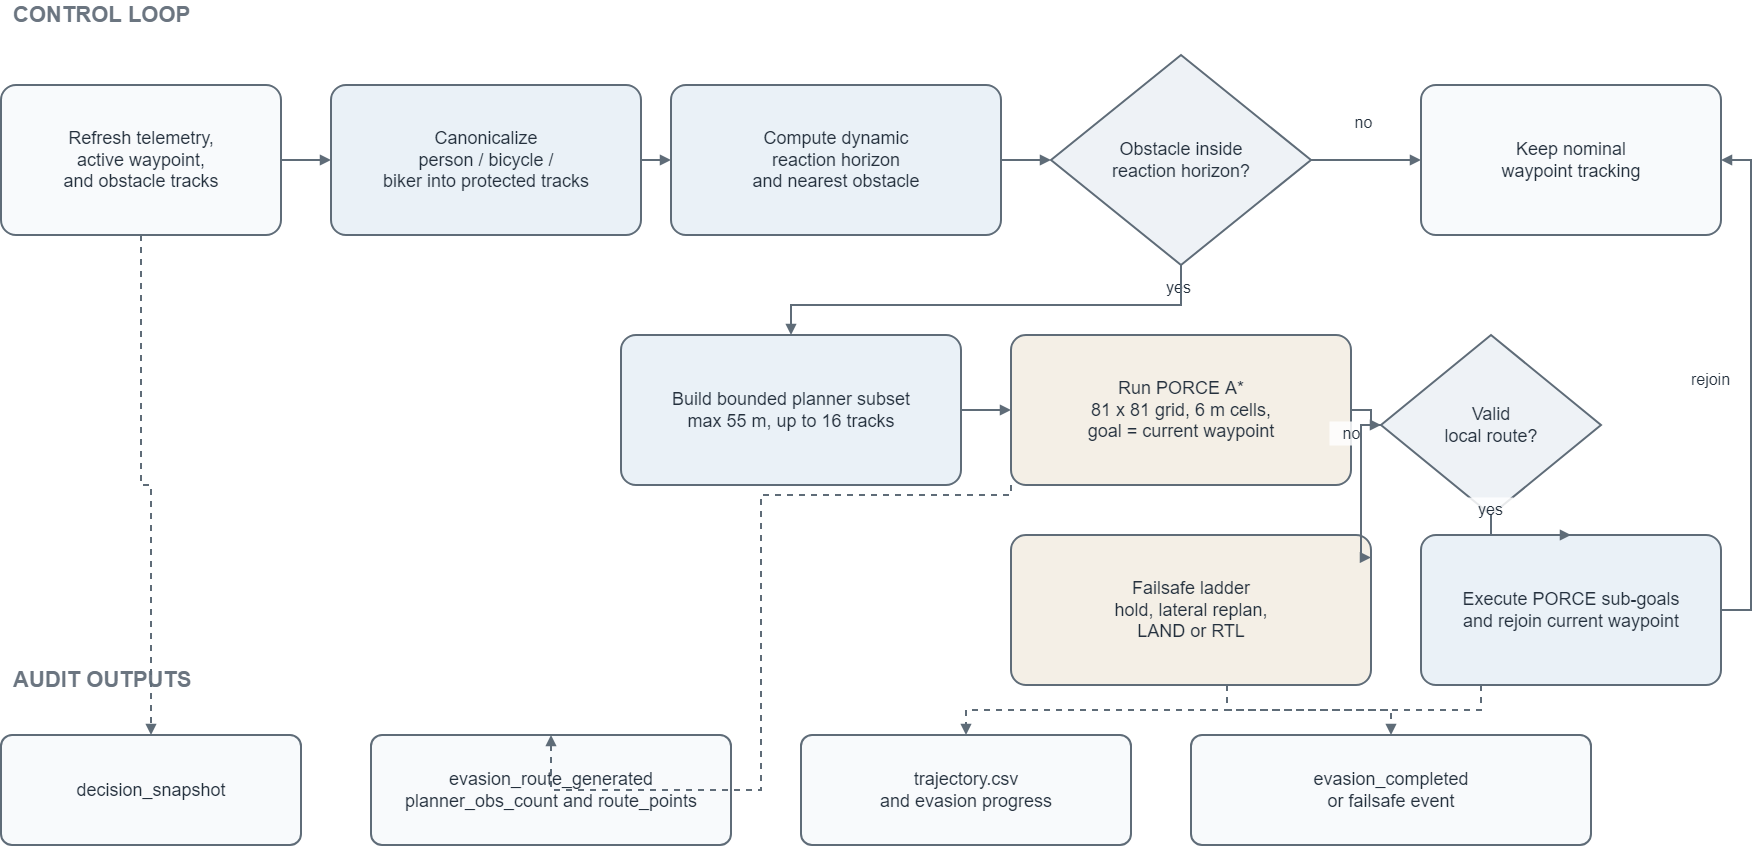
\includegraphics[width=\linewidth]{porce_method_flow.png}
    \caption{Controller-level PORCE decision flow. The same branch structure governs nominal tracking, local replanning, failsafe escalation, and audit event generation.}
    \label{fig:porce_method_flow}
\end{figure}

\subsection{Problem Formulation}

At each control iteration, the Brain knows the current vehicle state, the active mission waypoint, and the most recent obstacle list. The method is only concerned with the local subproblem: move from the current position to the current waypoint while avoiding the obstacle subset that lies inside a bounded planning neighborhood.

Let the vehicle position be \(p_t \in \mathbb{R}^2\), the current waypoint be \(w_t \in \mathbb{R}^2\), and the perceived obstacles at time \(t\) be \(\mathcal{O}_t = \{o_1,\dots,o_k\}\). Each obstacle is inflated by a hard safety radius \(R_s\), generating a non-flyable region
\begin{equation}
    \mathcal{Z}_{\mathrm{safe}}(o_i) = \{q \in \mathbb{R}^2 : \lVert q - p_{o_i} \rVert_2 \le R_s\}.
\end{equation}

The local free space is therefore
\begin{equation}
    \mathcal{F}_t = \mathbb{R}^2 \setminus \bigcup_{i=1}^{k} \mathcal{Z}_{\mathrm{safe}}(o_i).
\end{equation}

In the current implementation, \(R_s = \SI{12}{\meter}\), which turns safety into a hard geometric constraint instead of a soft penalty.

Earlier conceptual project notes also discussed more general continuous cost-shaping ideas, including barrier-style formulations, as possible future directions. They are not the subject of the present paper. The system analyzed here is the one actually implemented in the repository: a deterministic bounded grid planner with hard obstacle inflation and explicit failsafe escalation, not a Control Barrier Function controller or any other unimplemented continuous optimizer.

\subsection{Dynamic Triggering Logic}

The method is not permanently active. The controller computes a dynamic reaction horizon
\begin{equation}
    D_{\mathrm{react}}(t) =
    \mathrm{clip}\!\left(D_{\mathrm{base}} + k_v \lVert v_t \rVert_2,\,
    D_{\min},\, D_{\max}\right),
\end{equation}
where \(D_{\mathrm{base}}=\SI{45}{\meter}\), \(k_v=\SI{2.0}{\second}\), \(D_{\min}=\SI{45}{\meter}\), and \(D_{\max}=\SI{80}{\meter}\).

If the nearest perceived obstacle satisfies
\begin{equation}
    d_{\mathrm{nearest}}(t) \le D_{\mathrm{react}}(t),
\end{equation}
and the minimum replan interval has elapsed, the Brain requests a new local route from the replanning module. Otherwise, the vehicle continues nominal waypoint following.

\subsection{Bounded Local A* Planner}

The method uses a local occupancy grid centered on the vehicle. The validated configuration uses \(81 \times 81\) cells with \(\delta=\SI{6}{\meter}\) resolution, yielding a bounded search window that is compatible with online execution inside the control loop.

Each cell \(c_{ij}\) is labeled as free or occupied according to the inflated obstacle set:
\begin{equation}
    S(c_{ij}) =
    \begin{cases}
        1, & \text{if } c_{ij} \cap \left(\mathbb{R}^2 \setminus \mathcal{F}_t\right) \neq \varnothing,\\
        0, & \text{otherwise.}
    \end{cases}
\end{equation}

The local route is computed with A* \cite{hart1968formal} using Euclidean heuristic,
\begin{equation}
    f(n) = g(n) + h(n),
\end{equation}
where \(g(n)\) is the accumulated path cost and \(h(n)\) is the Euclidean distance to the local goal. Eight-connectivity is enabled, so the method can combine cardinal and diagonal moves while remaining on the grid.

The target of the method is always the \emph{current mission waypoint}. This detail is important: the local planner is not allowed to redefine the global mission, only to create a temporary bypass that lets the UAV return to the original corridor as soon as the conflict disappears.

\subsection{Nominal Navigation, Temporary Inhibition, and Route Reattachment}

One of the clearest implementation ideas in the repository is that the method should be understood as a \emph{temporary inhibition} of nominal navigation rather than as a new mission planner. When no relevant obstacle is detected, the Brain executes standard waypoint following: it keeps the current mission waypoint as target, checks whether the waypoint-tolerance condition is satisfied, and then advances to the next waypoint in the mission file. If the last waypoint is completed, the mission terminates normally through the landing logic.

When the nearest obstacle crosses the dynamic reaction horizon, this nominal flow is suspended and an evasion path becomes the active short-horizon reference. During that interval, the aircraft no longer tries to cut through the original corridor; instead, it follows the local sub-goals returned by the bounded A* planner. As soon as that local path is exhausted, nominal waypoint following resumes automatically toward the same mission waypoint that was active before the conflict. This point is operationally important for inspection: the objective of the method is not just to avoid collision, but to resolve the local conflict while returning as quickly as possible to the globally planned route that was originally chosen to optimize data capture and mission progression.

\subsection{Failsafe Escalation}

If no valid local route is found, the Brain does not continue nominal flight blindly. Instead, the system integration includes an explicit escalation chain with hold, lateral replan, and terminal \texttt{LAND}/\texttt{RTL} actions. This failsafe design is part of the method even when it is not triggered in a particular experiment because it bounds the controller behavior under planner failure.

\subsection{Algorithmic Summary}

\begin{algorithm}[t]
    \caption{Simplified control loop for the proposed method integrated in Pipeline A}
    \label{alg:replanner}
    \small
    \begin{algorithmic}[1]
        \While{mission is active}
            \State refresh telemetry, obstacle tracks, and current waypoint
            \If{telemetry is stale}
                \State \textbf{continue}
            \EndIf
            \If{failsafe action is active}
                \State execute failsafe and \textbf{continue}
            \EndIf
            \State compute \(D_{\mathrm{react}}(t)\) from current speed
            \State obtain nearest obstacle and planner obstacle subset
            \If{\(d_{\mathrm{nearest}}(t) \le D_{\mathrm{react}}(t)\) and replanning is allowed}
                \State route \(\gets\) A* local plan toward current mission waypoint
                \If{route is valid}
                    \State activate evasion path
                \Else
                    \State escalate failsafe
                \EndIf
            \EndIf
            \If{evasion path is active}
                \State follow next local replanning sub-point
            \Else
                \State follow nominal mission waypoint
            \EndIf
        \EndWhile
    \end{algorithmic}
\end{algorithm}

\section{Experimental Methodology}

\subsection{Evidence Sources}

The paper uses three complementary evidence sources present in the repository.
\begin{itemize}[leftmargin=1.3em]
    \item \textbf{Controlled E2E ablations:} a statistical campaign of 40+ mission logs from \texttt{pipeline/logs/e2e/} (ten or more runs per scenario) comparing the replanning module enabled or disabled, with and without detections, plus the four original representative logs.
    \item \textbf{Audited case study:} one clean zero-trust run (\texttt{20260612\_233504}) executed against the live Unreal Engine 5.7 digital-twin viewer, with trajectory logs, Brain events, per-frame vision audit payloads, and pristine archived viewer frames.
\end{itemize}

The E2E ablation isolates the behavioral effect of enabling the method under detections. The zero-trust run provides richer observability: trigger distance, generated route length, evasion duration, obstacle tracks, and the complete time evolution of the maneuver. The event \texttt{evasion\_route\_generated} now serializes both \texttt{planner\_obs\_count} and the exact obstacle identities (\texttt{planner\_obs\_ids}) passed to the planner, so the clearance analysis in this paper is computed against the audited planner subset itself rather than a proxy. Because the trigger-side obstacles in the case study are moving cyclists, clearance is evaluated against the concurrently published track positions at each instant of the maneuver, as recorded by the perception audit stream.

\subsection{Mission and Metrics}

The mission comes from \texttt{pipeline/ejea\_default.waypoints}. It contains a takeoff waypoint, a sequence of inspection waypoints, and a landing command. For all experiments, the UAV climbs from \SI{500}{\meter} MSL to approximately \SI{523}{\meter} MSL, follows the inspection corridor, and lands autonomously once the final waypoint is reached.

The following metrics are extracted from logs:
\begin{itemize}[leftmargin=1.3em]
    \item mission duration, measured from the first to the last status sample in the E2E logs;
    \item path length, computed by summing point-to-point geodesic distances along the logged trajectory;
    \item trigger distance, route-point count, and evasion duration from \texttt{events.jsonl};
    \item minimum time-synchronized separation between the executed evasion trajectory and the concurrently published tracks of the trigger-side obstacle class;
    \item detour cost, computed as the difference between evasion path length and the straight-line segment joining the first and last evasion points.
\end{itemize}

The visual materials discussed in the paper were generated directly from repository logs by a dedicated script placed inside the \texttt{paper/} folder. The generated assets include the system architecture, the controller flow, the E2E ablation plot, the YOLO perception overlay, the six-stage collision-evasion sequence, the metric audit montage, the executed local trajectory, and the clearance time series. This keeps the visual evidence reproducible from project artifacts rather than manually drawn after the fact.

\section{Experimental Validation of the Proposed Method}

\subsection{Controlled E2E Ablation}

Figure~\ref{fig:e2e_ablation} shows the early section of the E2E trajectories. The two scenarios without detections are practically identical regardless of whether the replanning module is enabled, which confirms that the planner remains dormant when no conflict enters the system. The \texttt{replanner off + detections} scenario also follows the nominal corridor, while \texttt{replanner on + detections} introduces a visible local detour before rejoining the original path.

\begin{figure}[t]
    \centering
    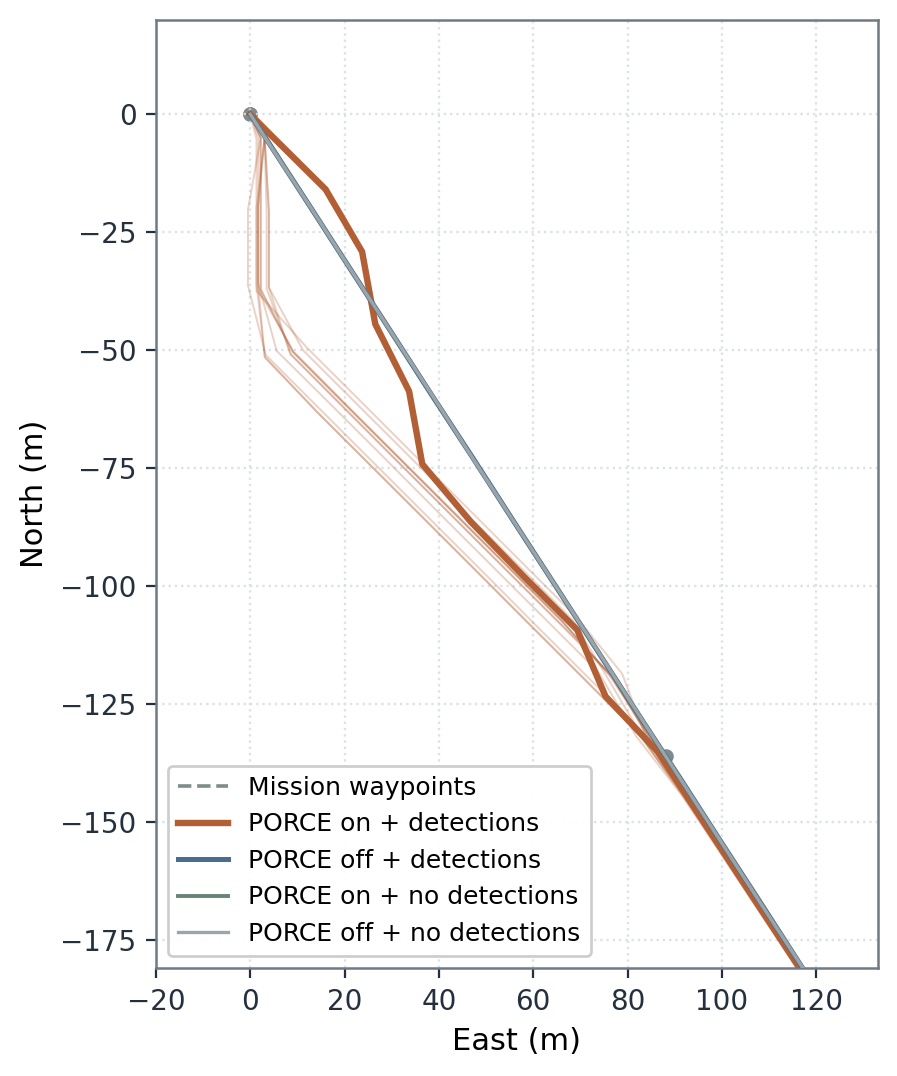
\includegraphics[width=0.88\linewidth]{e2e_ablation_paths.png}
    \caption{Controlled E2E trajectory ablation. Only the configuration with detections and PORCE enabled introduces a local detour, while the other three scenarios remain on the nominal corridor.}
    \label{fig:e2e_ablation}
\end{figure}

Table~\ref{tab:e2e} quantifies this result over the full statistical campaign (ten or more runs per scenario, all missions completed). The overhead introduced by the avoidance behavior is small and stable: relative to \texttt{replanner off + detections}, enabling the method under detections adds on average \SI{8.3}{\meter} to the path and \SI{2.1}{\second} to the total mission, with sub-meter and sub-second standard deviations in the unperturbed scenarios.

\begin{table}[t]
    \centering
    \caption{Controlled E2E ablation metrics extracted from \texttt{pipeline/logs/e2e} (mean $\pm$ standard deviation over the 2026-06-12 campaign).}
    \label{tab:e2e}
    \small
    \begin{tabularx}{\linewidth}{@{}Y c c c@{}}
        \toprule
        \textbf{Scenario} & {\textbf{Time (s)}} & {\textbf{Path (m)}} & \textbf{Completed} \\
        \midrule
        replanner on + detections & $207.1 \pm 0.3$ & $1463.8 \pm 1.4$ & 11/11 \\
        replanner off + detections & $205.0 \pm 0.0$ & $1455.5 \pm 0.2$ & 10/10 \\
        replanner on + no detections & $205.9 \pm 1.0$ & $1455.8 \pm 0.2$ & 10/10 \\
        replanner off + no detections & $206.8 \pm 1.0$ & $1455.7 \pm 0.2$ & 10/10 \\
        \bottomrule
    \end{tabularx}
\end{table}

Beyond aggregate cost, the campaign verifies an operationally important property of the proposed method: the system is behaviorally specific. Evasion activated in every run of the \texttt{replanner on + detections} scenario (11/11) and in none of the other three scenarios (0/30). The mission is perturbed only when both conditions hold simultaneously, namely obstacle evidence is present and the replanning module is enabled.

\subsection{Audited Collision-Evasion Maneuver}

The selected zero-trust maneuver comes from run \texttt{20260612\_233504}, executed against the live Unreal Engine 5.7 digital twin with a parametric sixteen-rider cycling peloton crossing the inspection corridor at \SI{23}{\kilo\meter\per\hour}. It is intentionally stricter than tower/cattle-like cases because the trigger-side detections are \texttt{biker} tracks, i.e. the human-adjacent obstacle family that most directly supports the no-overflight claim of the proposed method. At the trigger instant (vision frame 5728 at \(t=+\SI{0.032}{\second}\)), fifteen \texttt{biker} tracks are concurrently published by the perception stream, and the route event records sixteen planner obstacles together with their serialized identities (\texttt{planner\_obs\_ids}), so the planner subset used for the analysis is the audited one, not a reconstruction.

Figure~\ref{fig:yolo_future_overlay} gives the perceptual reading of the same event. The left panel shows the archived viewer frame captured at the trigger instant directly from the Unreal window, with the logged YOLO bounding boxes drawn on top from \texttt{events.jsonl}; boxes, track IDs, confidences, distances, frame counters, route length, and altitude values are all read back from the zero-trust logs. The right-hand panel reconstructs the ground-projected \texttt{biker} trace and a short linear forecast from logged detections rather than from generated imagery.

\begin{figure}[p]
    \centering
    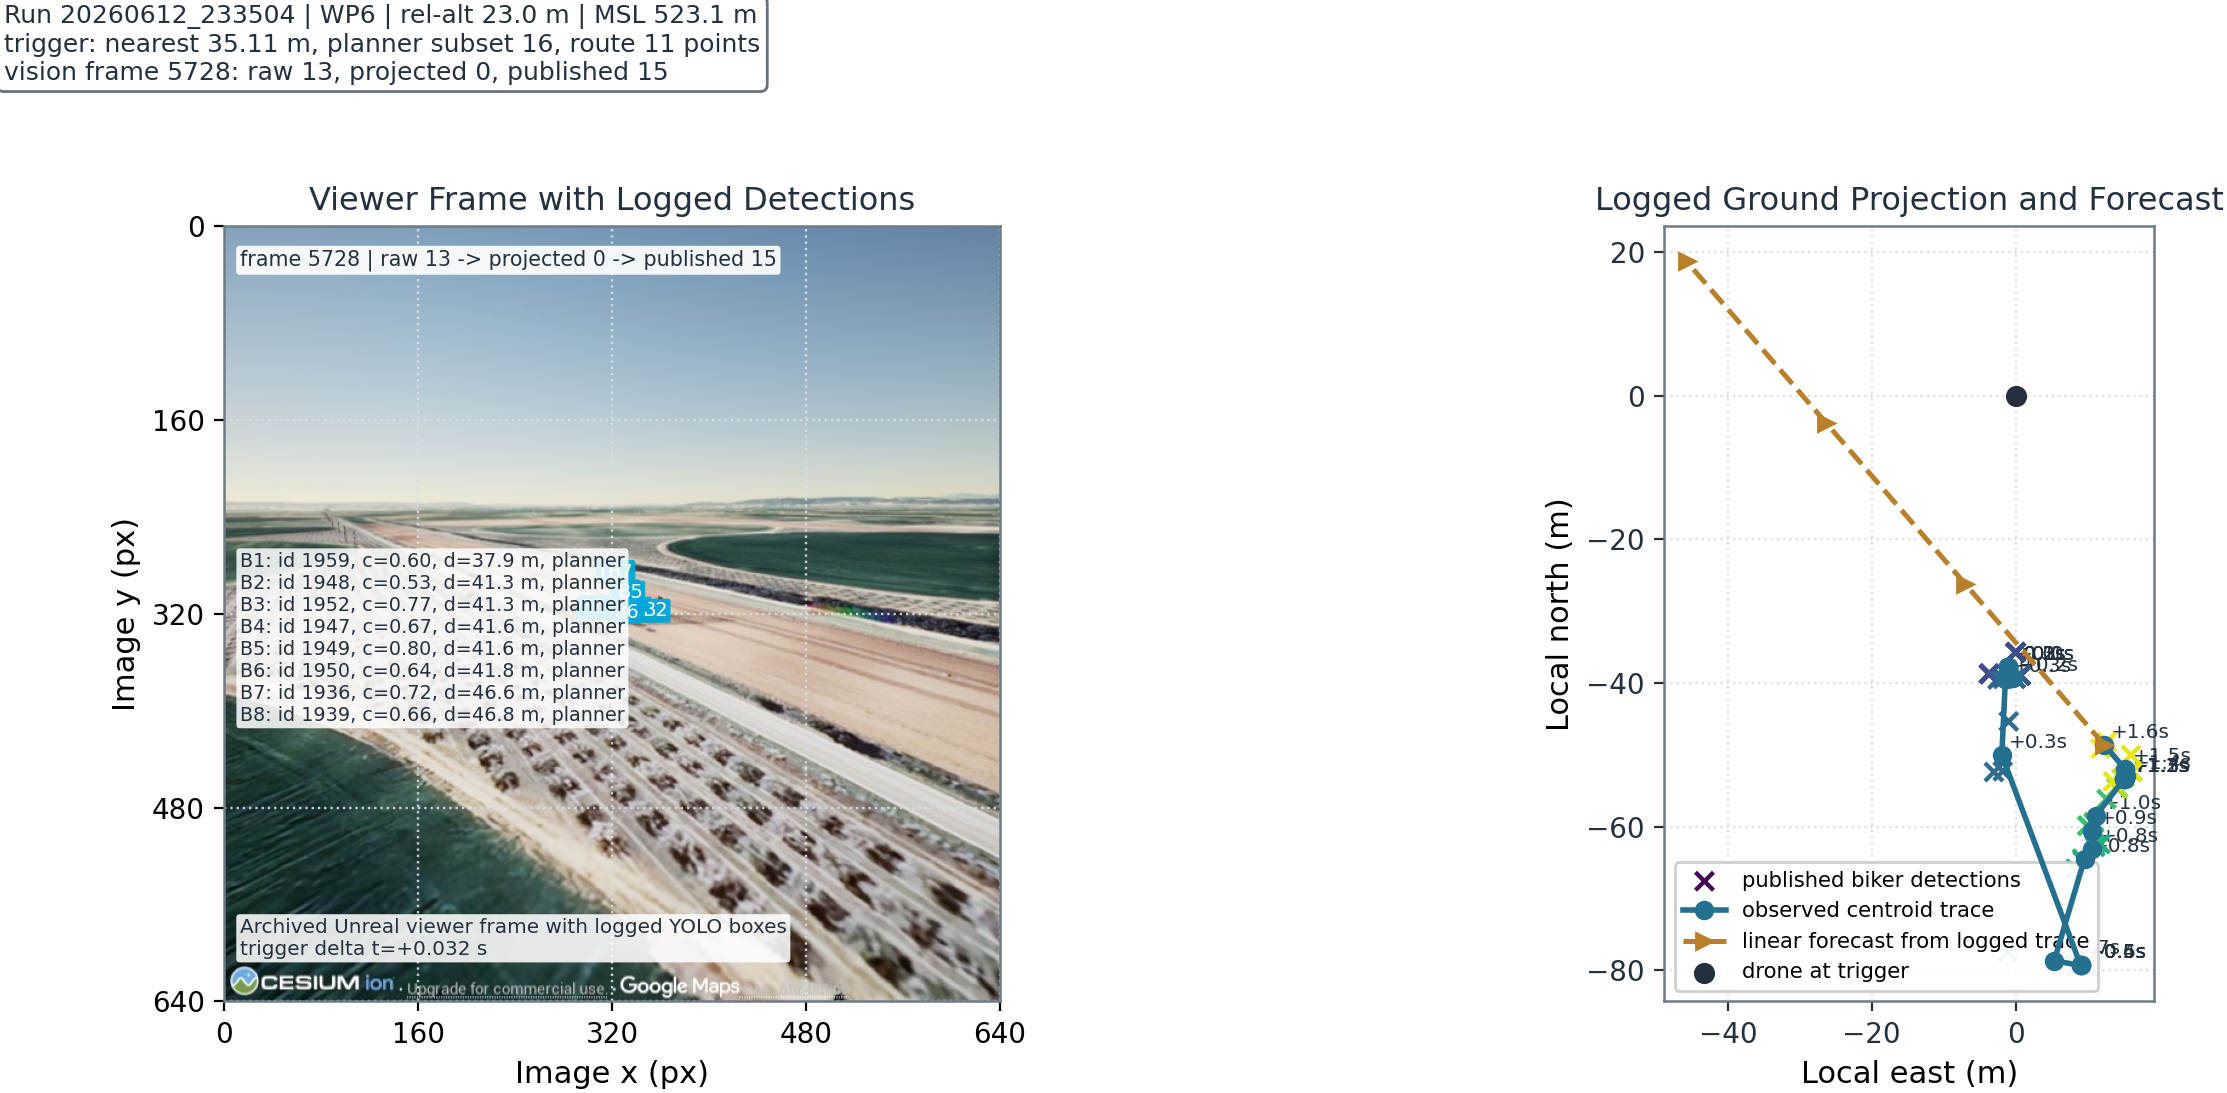
\includegraphics[width=\linewidth]{porce_yolo_future_overlay.png}
    \caption{Perception overlay for the audited maneuver. The left panel shows the archived Unreal viewer frame at the trigger instant with the logged YOLO bounding boxes drawn from the audit stream; the right panel uses the same detections after ground projection to show observed motion and a short scripted forecast.}
    \label{fig:yolo_future_overlay}
\end{figure}

Figure~\ref{fig:porce_six_stage} turns the maneuver into a six-stage operational sequence: obstacle detection, class labeling and track publication, distance and reaction-horizon evaluation, local bypass planning, online recalculation while detections evolve, and rejoining of the nominal mission corridor after the protected region has been passed.

\begin{figure}[p]
    \centering
    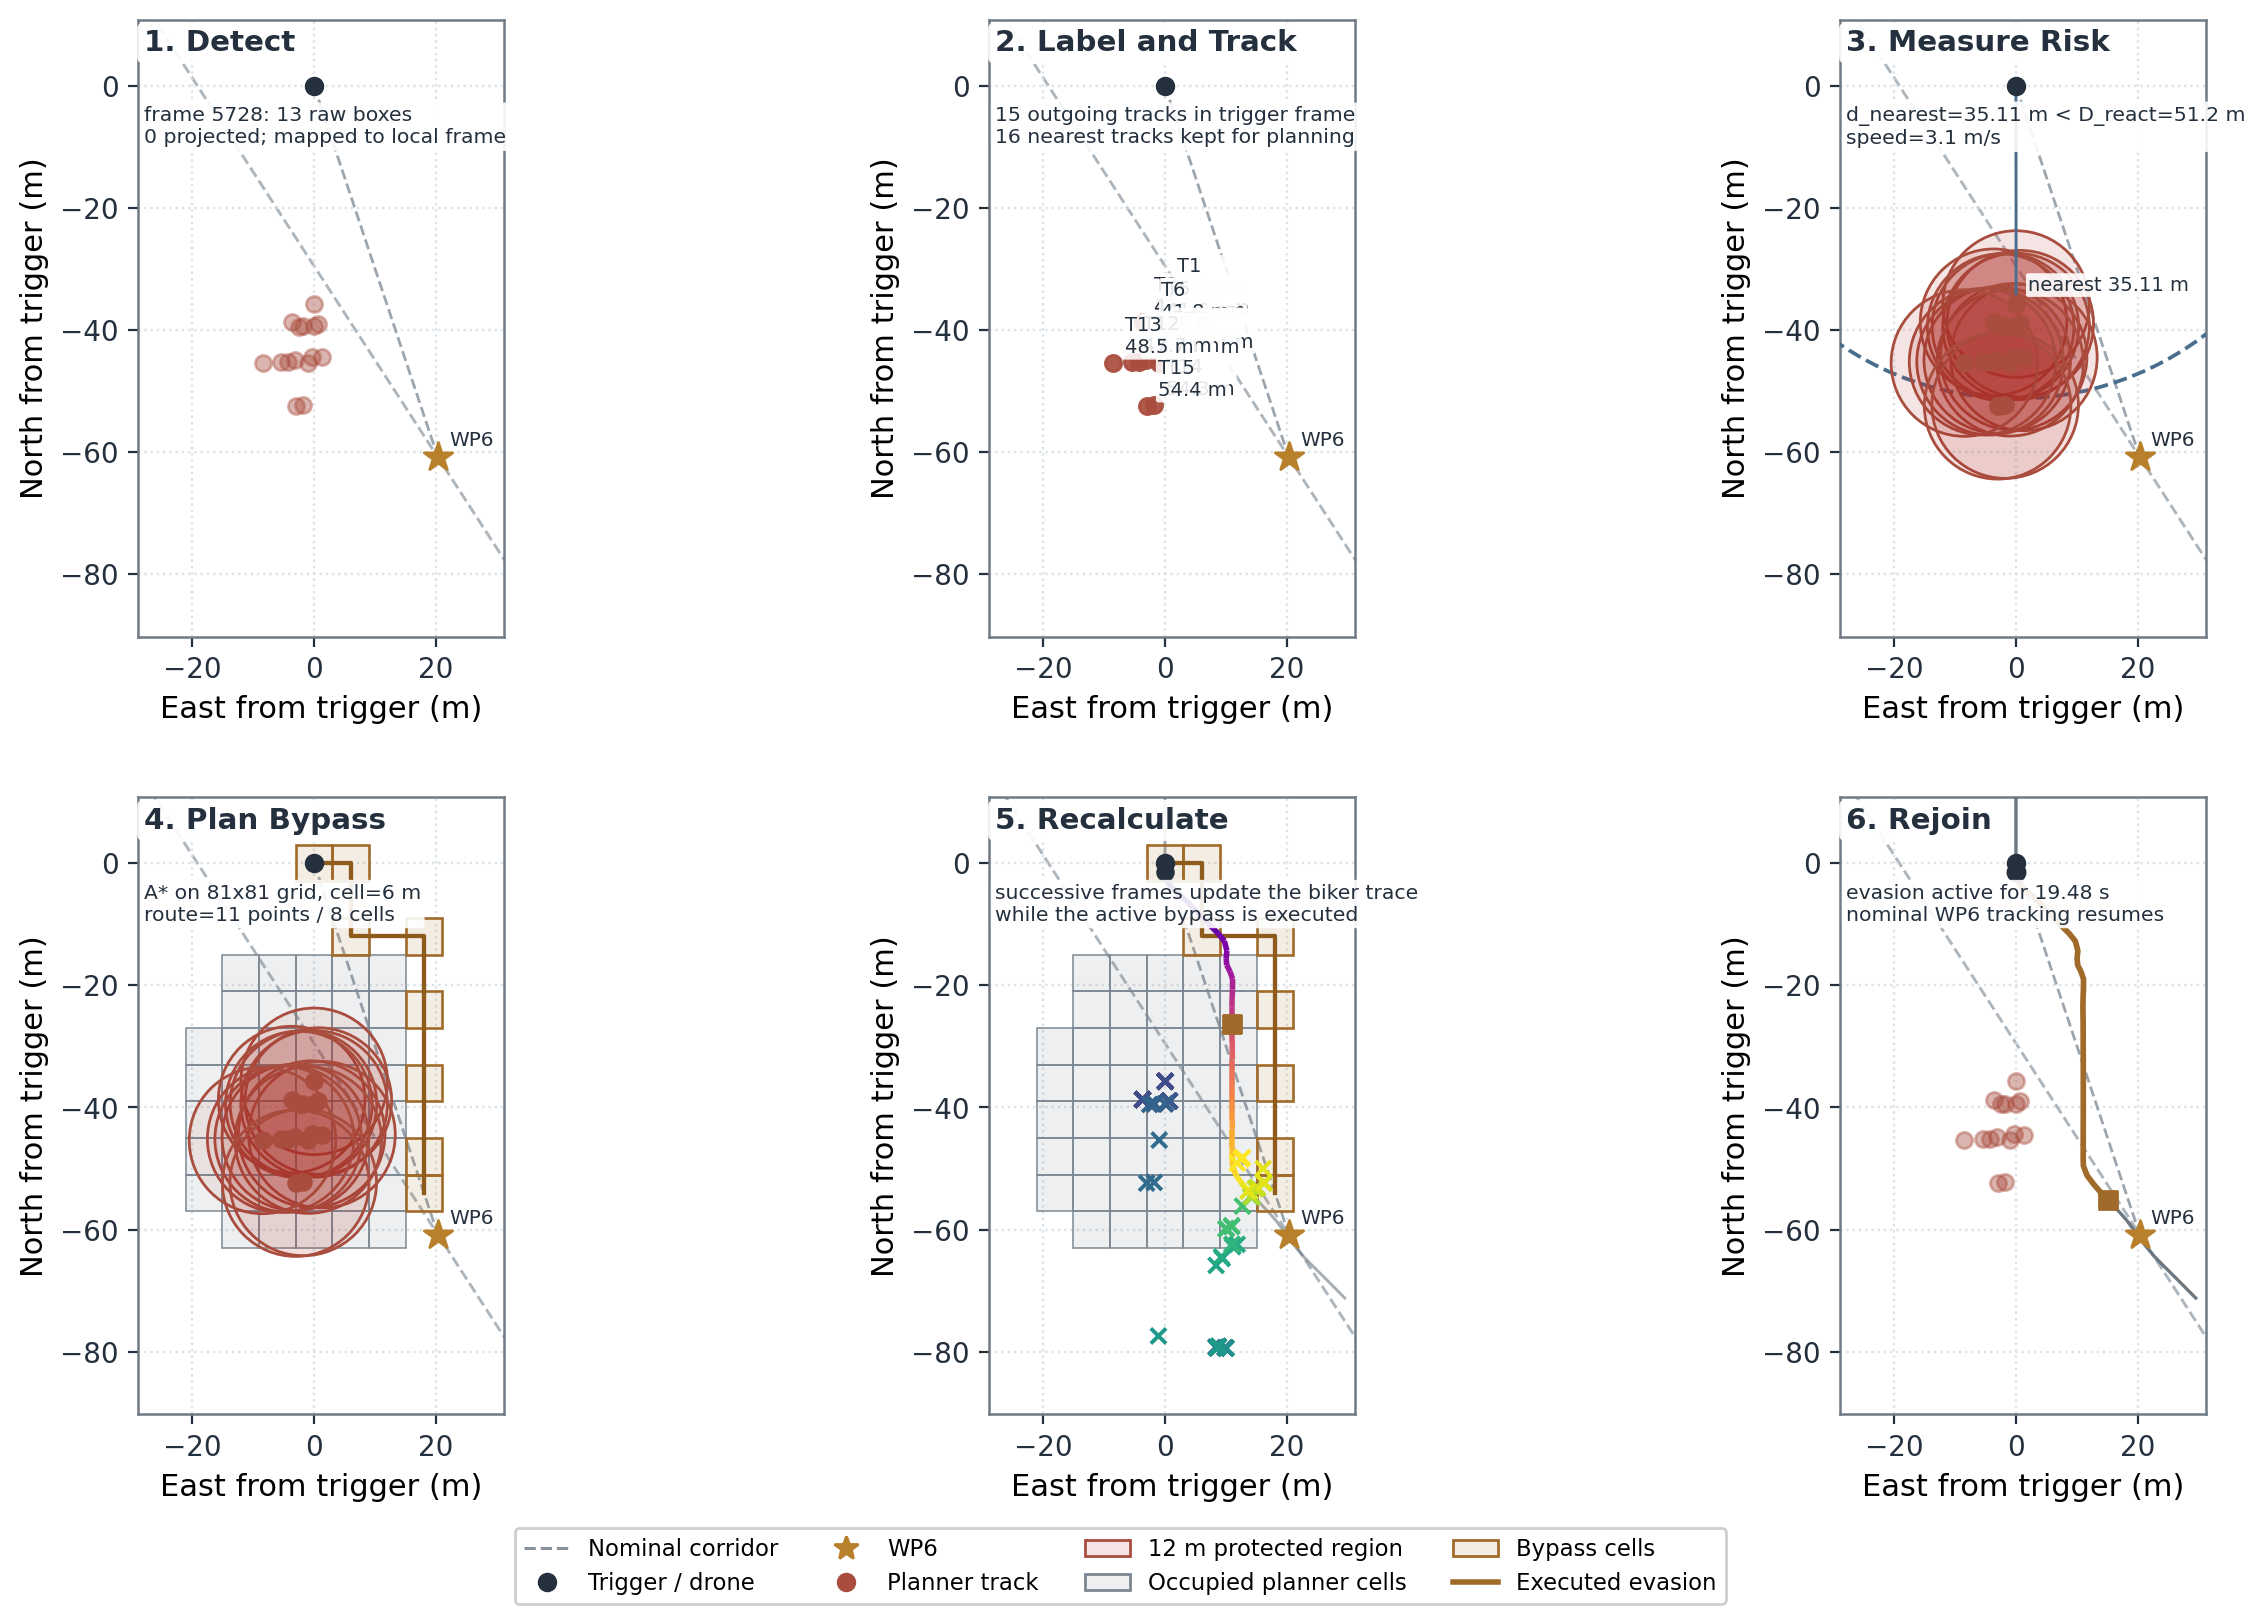
\includegraphics[width=\linewidth]{porce_six_stage_sequence.png}
    \caption{Six-stage reconstruction of the audited PORCE maneuver, from YOLO detection to nominal-route rejoin. All panels use the same local ENU view centered on the trigger state, while successive panels add the projected detections, planner subset, reaction horizon, discretized bypass, executed evasion, and final rejoin.}
    \label{fig:porce_six_stage}
\end{figure}

The perception-to-planner audit chain is shown in Figure~\ref{fig:porce_detection_montage}. The top row records the reduction from raw detector boxes to the planner subset, and the bottom row shows the same instant in pixel space, metric ENU space, and planner-grid space. This figure is primarily probative rather than illustrative: it shows how raw perception evidence becomes the bounded obstacle set that conditions route generation.

\begin{figure}[p]
    \centering
    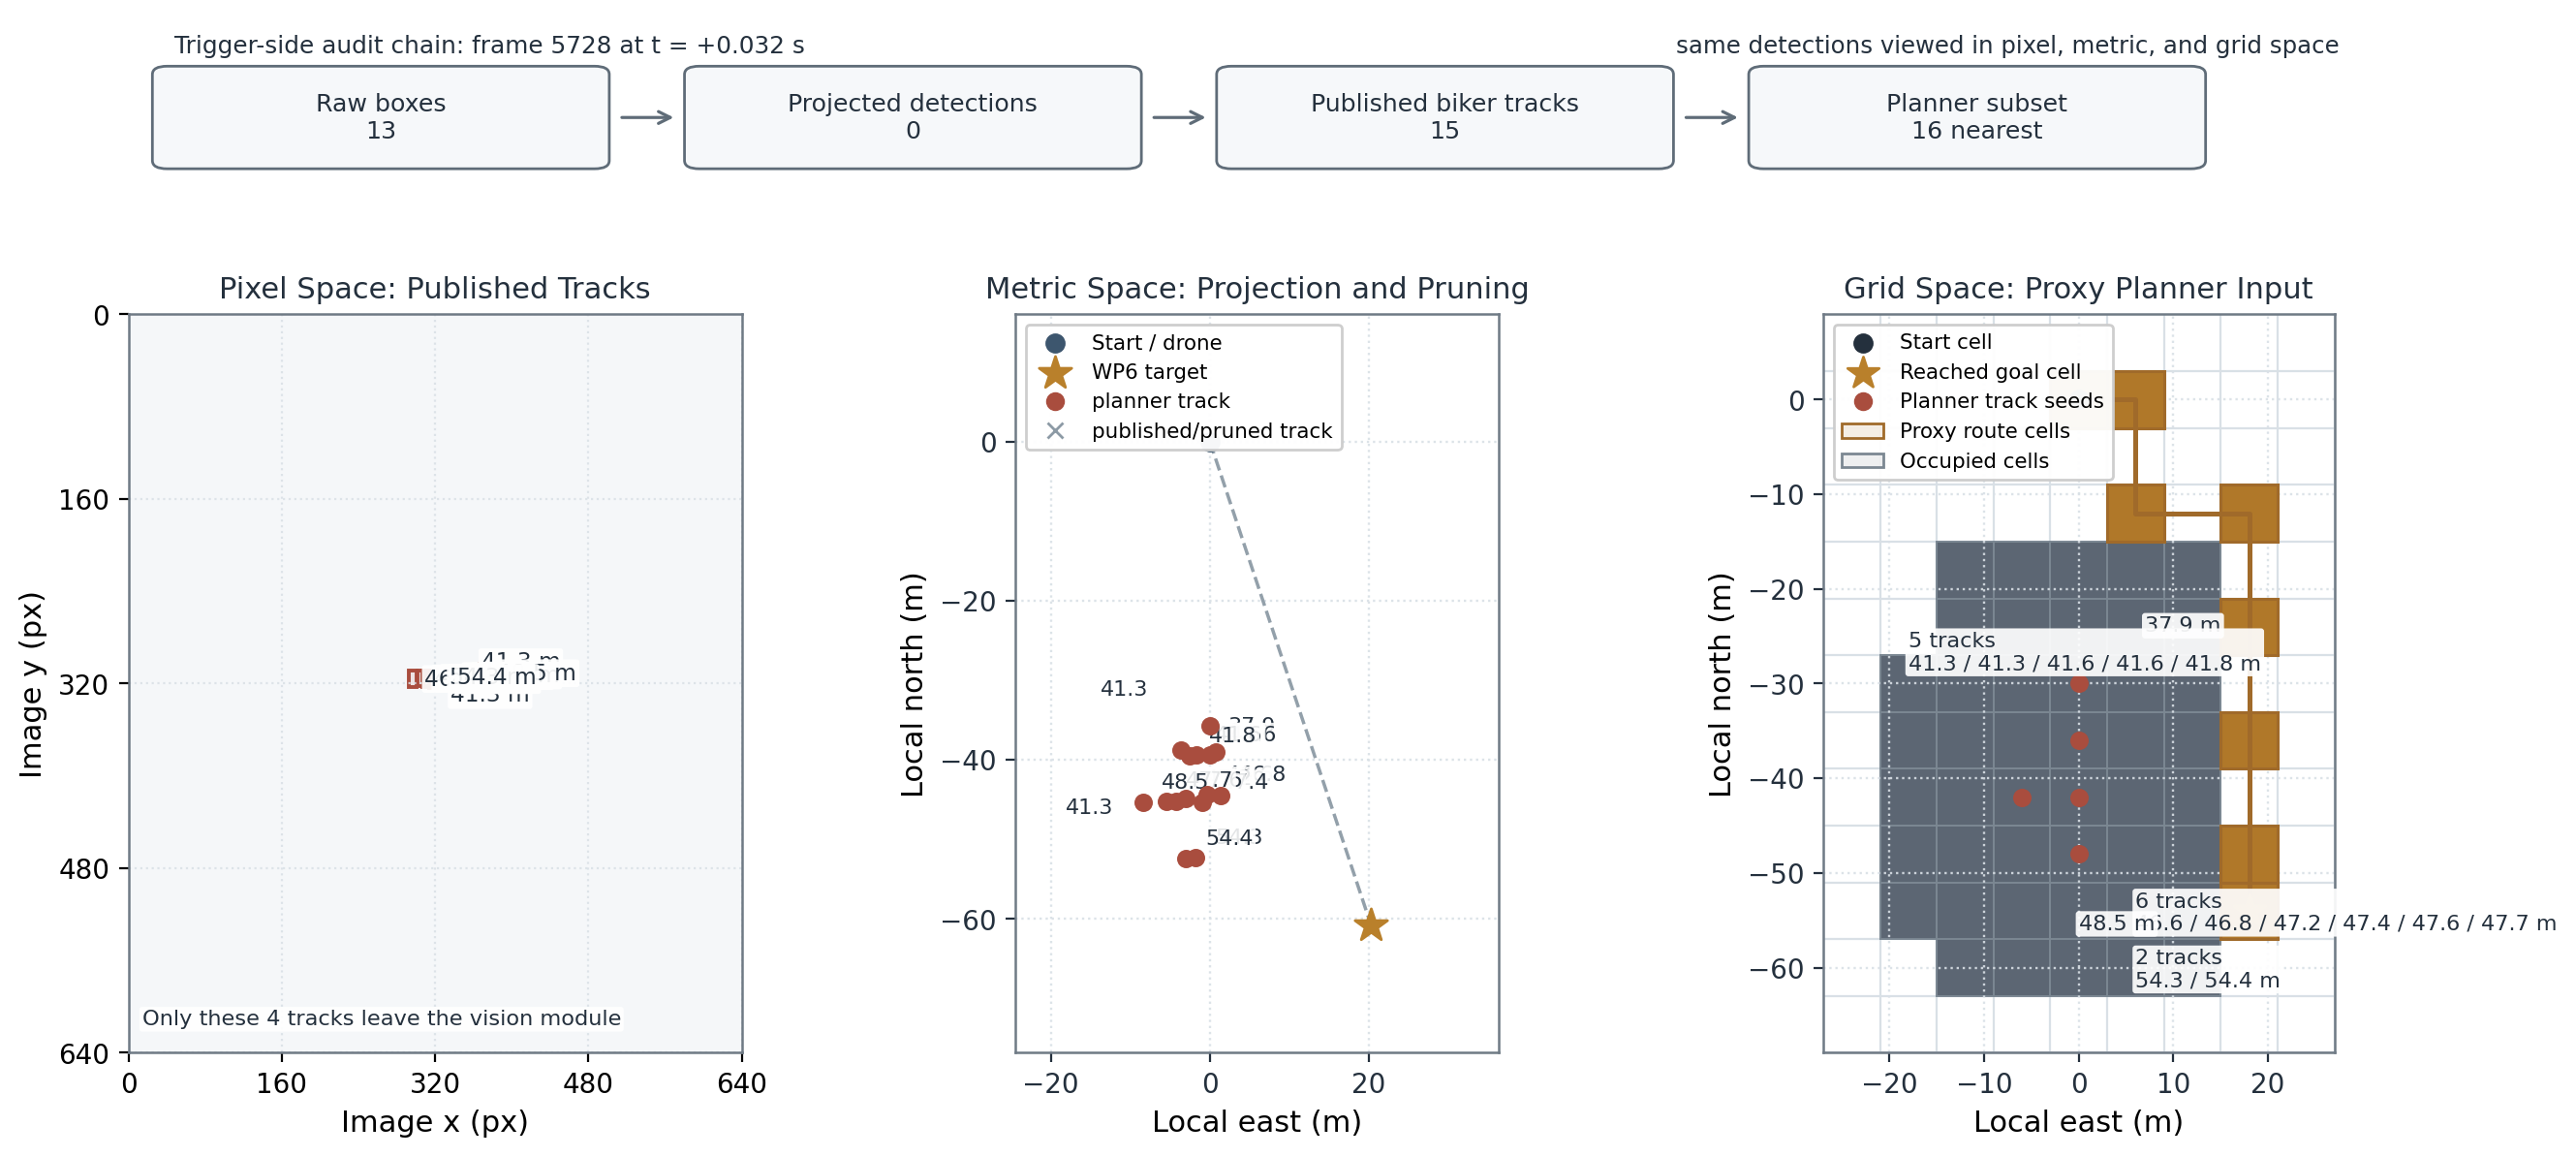
\includegraphics[width=\linewidth]{porce_detection_montage.png}
    \caption{Perception-to-planner audit chain for the trigger-side \texttt{biker} event. The same detections are displayed as camera boxes, local metric points, and inflated planner-grid cells.}
    \label{fig:porce_detection_montage}
\end{figure}

The geometric effect of the method in a local ENU frame centered on the trigger-side telemetry state is shown in Figure~\ref{fig:porce_case_trajectory}. The background lattice matches the real \SI{6}{\meter} planner discretization, while the shaded occupied cells correspond to the sixteen audited planner obstacles (serialized in \texttt{planner\_obs\_ids}) inflated with the configured \SI{12}{\meter} safety radius. Because the peloton rides in a compact formation, several tracks quantize to adjacent or shared seed cells, so the merged occupied blocks are a genuine property of the planner discretization rather than a drawing artifact. The vehicle departs from the nominal mission corridor, executes a bounded bypass around the moving group, and rejoins the original path before continuing toward WP6.

\begin{figure}[p]
    \centering
    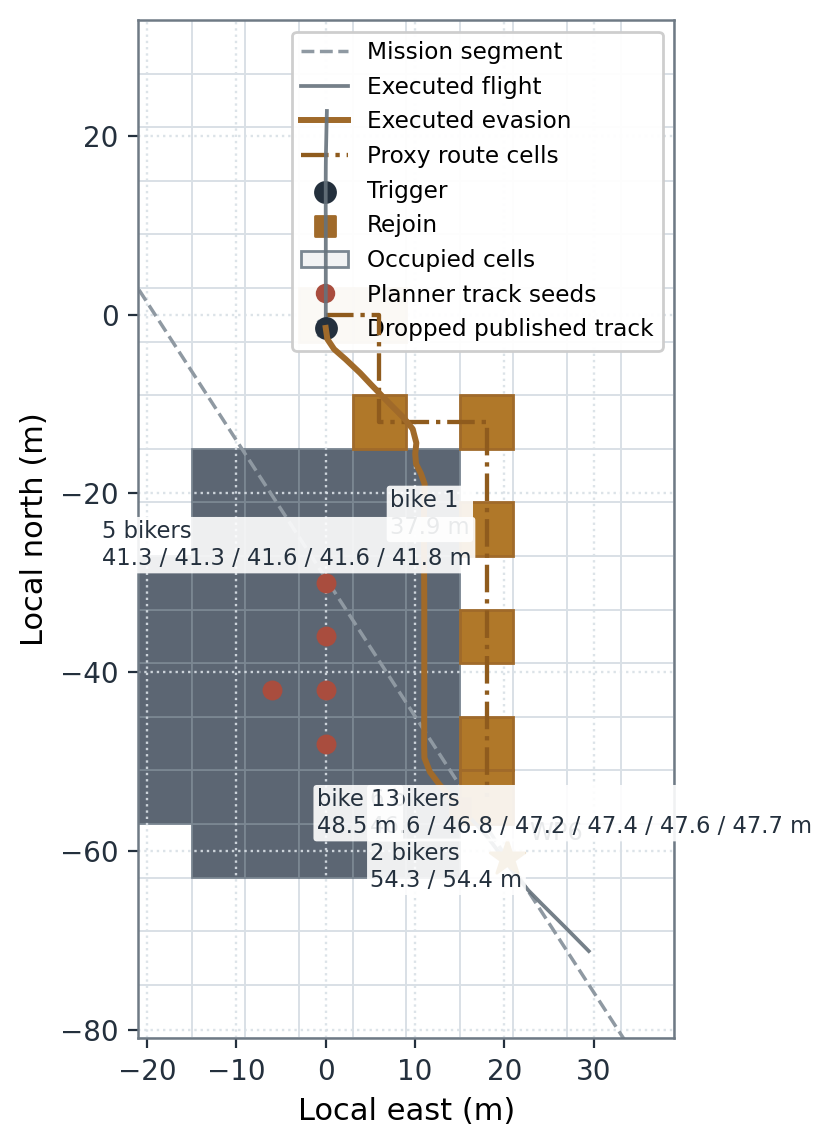
\includegraphics[width=0.82\linewidth]{porce_case_trajectory.png}
    \caption{Audited local trajectory of the PORCE case study. Occupied cells are generated by inflating the sixteen audited trigger-side planner obstacles, and the executed evasion rejoins the original mission segment.}
    \label{fig:porce_case_trajectory}
\end{figure}

The geometric view is complemented by Figure~\ref{fig:porce_case_timeseries}. Because the trigger-side obstacles are moving cyclists, the clearance signal is computed against the concurrently published track positions at each vision frame rather than against frozen trigger seeds. The reaction horizon remains active throughout the event, and the time-synchronized clearance never drops below \SI{34.3}{\meter}: the maneuver keeps the vehicle not only outside the hard \SI{12}{\meter} safety radius but also above the \SI{22}{\meter} failsafe threshold for the entire \SI{19.5}{\second} engagement with the peloton.

\begin{figure}[p]
    \centering
    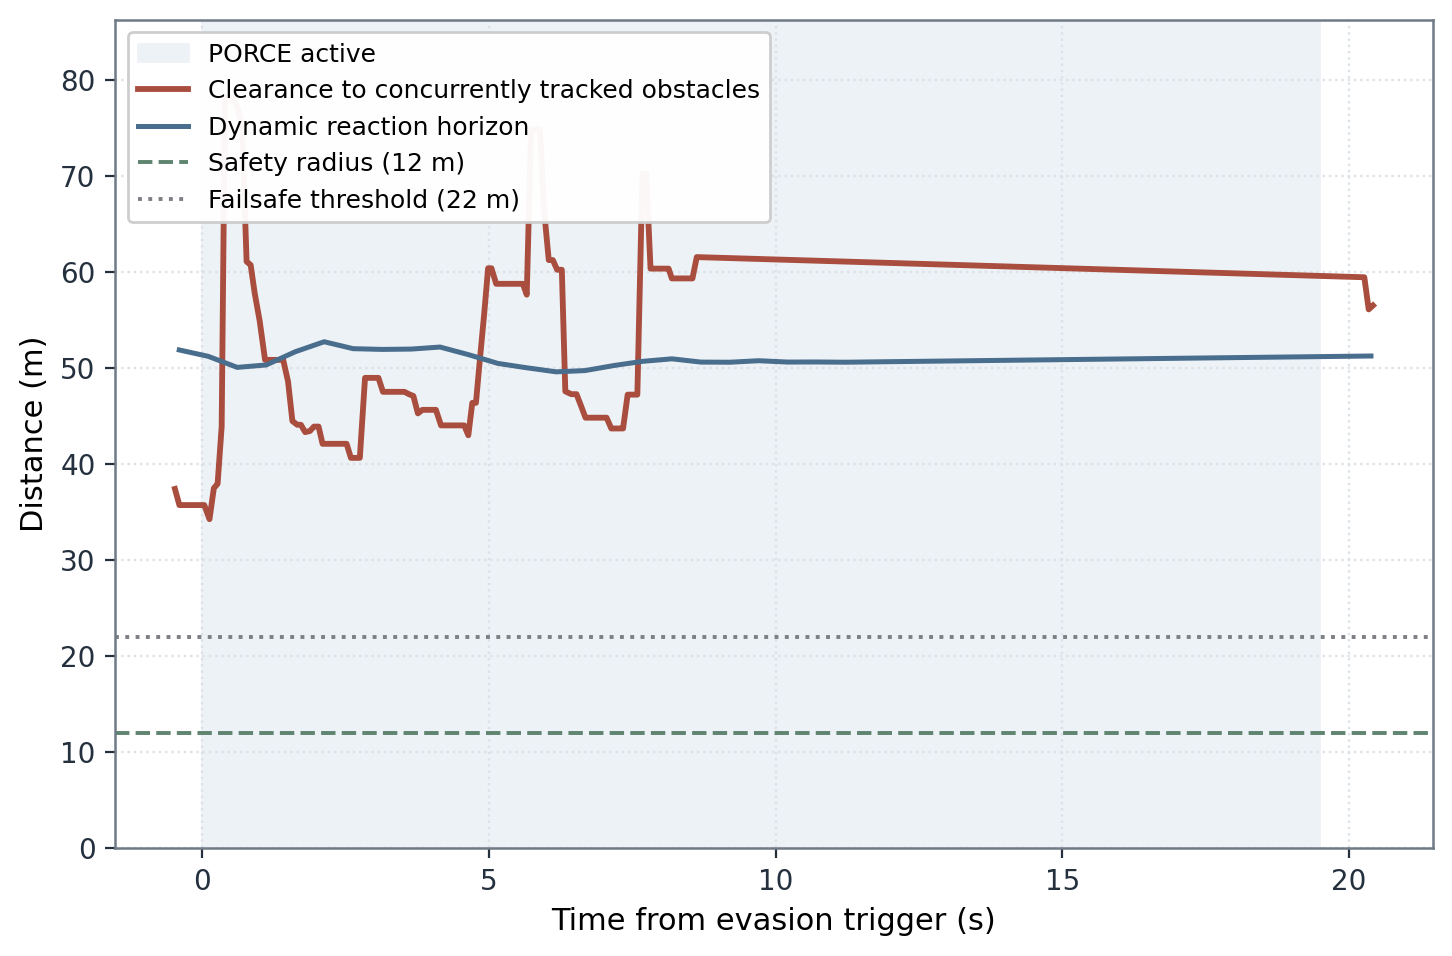
\includegraphics[width=0.86\linewidth]{porce_case_timeseries.png}
    \caption{Clearance and reaction-distance time series for the audited maneuver. The time-synchronized clearance to concurrently tracked obstacles remains above both the configured \SI{12}{\meter} hard safety radius and the \SI{22}{\meter} failsafe threshold while the local evasion route is active.}
    \label{fig:porce_case_timeseries}
\end{figure}

Table~\ref{tab:case} summarizes the main metrics derived from the audited run. The method is triggered at \SI{35.11}{\meter}, well inside the observed reaction horizon. It computes an 11-point local route and completes the maneuver in \SI{19.48}{\second}, during which the planner is re-seeded online as the peloton advances. The evasion path length is \SI{59.17}{\meter}; the equivalent straight-line segment between the first and last evasion points is \SI{55.75}{\meter}, so the local safety maneuver introduces a detour of only \SI{3.42}{\meter}. Most importantly, the minimum time-synchronized separation to the concurrently tracked \texttt{biker} positions is \SI{34.27}{\meter}, i.e. \SI{22.27}{\meter} of margin above the configured safety radius, sustained against a moving group of fifteen published human-adjacent tracks.

\begin{table}[t]
    \centering
    \caption{Main audited metrics for run \texttt{20260612\_233504}.}
    \label{tab:case}
    \small
    \begin{tabularx}{\linewidth}{@{}Y S[table-format=3.2]@{}}
        \toprule
        \textbf{Metric} & {\textbf{Value}} \\
        \midrule
        Trigger distance (m) & 35.11 \\
        Published \texttt{biker} tracks in pre-trigger frame & 15 \\
        Audited planner obstacles (\texttt{planner\_obs\_ids}) & 16 \\
        Local route points & 11 \\
        Evasion duration (s) & 19.48 \\
        Maximum reaction distance during maneuver (m) & 52.73 \\
        Minimum concurrent clearance to tracked \texttt{biker}s (m) & 34.27 \\
        Clearance above safety radius (m) & 22.27 \\
        Evasion path length (m) & 59.17 \\
        Straight-line equivalent (m) & 55.75 \\
        Local detour over straight segment (m) & 3.42 \\
        \bottomrule
    \end{tabularx}
\end{table}

The behavior is not specific to a single favorable pass. A verification run executed with a denser and slower peloton configuration (sixteen riders at a realistic \SI{23}{\kilo\meter\per\hour}) produced 94 \texttt{biker}-class replanning events distributed across the full inspection corridor (waypoints 3 through 10), eight completed evasion cycles, and still finished the mission and landed autonomously, which supports the robustness of the detect--replan--rejoin loop along the whole route rather than at an isolated crossing.

The zero-trust logs also allow a first characterization of the perception-to-planner latency on the workstation used for the experiments. Over the audited run, the vision loop (window capture, YOLO inference, projection, tracking, and publication) sustains a median period of \SI{69}{\milli\second} (14.6 frames per second, $p_{95}=\SI{90}{\milli\second}$); the median time between the first publication of a new obstacle track and its first appearance in an audited planner subset is \SI{0.62}{\second} ($p_{95}=\SI{3.7}{\second}$, dominated by tracks published while a replan-interval hold is active); and the replan cadence while engaged is \SI{1.01}{\second}, matching the configured \SI{1.0}{\second} minimum replan interval. These are workstation measurements intended as an auditable baseline rather than as onboard performance claims.

Taken together, the ablation and the audited case study support two claims. First, the method is selective: it does not inject unnecessary motion when obstacle evidence is absent. Second, when it does intervene, it produces a bounded and interpretable geometric deviation rather than a wholesale mission rewrite. For a power-line inspection workflow, this combination of selectivity, recoverability, and auditability is at least as important as raw avoidance capability.

\section{Limitations and Future Work}

The current paper is intentionally aligned with the evidence already available for the proposed method in the repository, and this imposes clear limits on what can be claimed.
\begin{itemize}[leftmargin=1.3em]
    \item The experiments are simulation-based. The method is validated in Pipeline A under \texttt{SIMULATION}, but the real-world workflow still requires dedicated flight campaigns.
    \item The quantitative section is reproducible and now statistical for the controlled ablation (ten or more runs per scenario with mean and standard deviation), but it is still a single-mission benchmark: broader scenario diversity (different corridors, obstacle densities, and weather/lighting conditions) remains future work.
    \item The regulatory novelty is operational rather than juridically complete. The method currently approximates uninvolved civilians through human-adjacent dynamic obstacle classes and conservative geometric avoidance; it is not yet a full SORA-compliant optimizer with class-dependent legal mitigations.
    \item The exact planner obstacle identities are serialized in \texttt{evasion\_route\_generated} (field \texttt{planner\_obs\_ids}) as of the 2026-06-12 audit patch, and the case study uses them directly. Archived runs recorded before that patch only expose \texttt{planner\_obs\_count}, so any retrospective analysis of older logs still requires the nearest-track proxy.
    \item Perception uncertainty is only partially represented through the detector and geopositioning chain. Future experiments should characterize measurement error, missed detections, and class-dependent inflation policies more rigorously.
\end{itemize}

The next development steps are therefore clear: integrate broader scenario sets, add runtime measurements on representative onboard hardware, encode class-dependent safety envelopes for humans and other critical entities, and transfer the same audited methodology to the \texttt{REAL\_TWIN} and real-flight workflows.

\section{Conclusion}

This paper turns Path Planning and Obstacle Avoidance Real-Time Collision Evasion into the explicit scientific center of the manuscript and grounds its characterization on repository evidence. The method is a bounded A* local replanning method that reacts only when necessary, preserves conservative geometric margins, and returns to the global mission once the conflict is resolved. Its specific contribution is not to claim that obstacle avoidance itself is novel, but to show how a local replanner can be shaped by the European ground-risk logic that discourages exposing uninvolved people and protected ground areas to unnecessary overflight. Pipeline A, in turn, provides the integrated simulation environment in which this behavior can be observed, audited, and measured.

The controlled E2E ablation shows, over ten or more runs per scenario, that the overhead of enabling the method under detections is small and stable, while the audited case study demonstrates that the method can generate and execute a complete local bypass around a moving group of fifteen tracked human-adjacent obstacles while sustaining an explicit, time-synchronized safety margin above the configured protection radius. Therefore, the strongest publishable claim is also the most precise one: to the best of our knowledge after reviewing recent 2024--2026 literature, the method represents the current state of the art for the narrowly defined problem of EASA-motivated, uninvolved-people-aware, deterministic controller-level local replanning inside an autonomous power-line inspection pipeline. Stated this way, the claim is ambitious but not misleading, because it does not assert superiority over all avoidance planners or all risk-aware route optimizers; it asserts leadership in the specific intersection that the system actually implements and documents.

\begin{thebibliography}{99}
\bibitem{imran2025environmental}
Imran and J. Li. ``Environmental and economic impact of UAV technology in agriculture''. in \emph{UAV Aerodynamics and Crop Interaction: Revolutionizing Modern Agriculture with Drone}, pp. 389--429, Springer, 2025. doi: \url{10.1007/978-981-96-8402-1_12}.
\bibitem{marut2024surveillance}
A. Marut, P. Wojciechowski, K. Wojtowicz, J. Djabin, J. Kochan, and M. Kurenda. ``Surveillance and protection of critical infrastructure with Unmanned Aerial Vehicles''. in \emph{2024 IEEE International Workshop on Technologies for Defense and Security (TechDefense)}, IEEE, pp. 312--317, 2024. doi: \url{10.1109/TechDefense63521.2024.10863159}.
\bibitem{debnath2024review}
D. Debnath, F. Vanegas, J. Sandino, A. F. Hawary, and F. Gonzalez. ``A review of UAV path-planning algorithms and obstacle avoidance methods for remote sensing applications''. \emph{Remote Sensing}, vol. 16, no. 21, pp. 4019, 2024. doi: \url{10.3390/rs16214019}.
\bibitem{meng2025advances}
W. Meng, X. Zhang, L. Zhou, H. Guo, and X. Hu. ``Advances in UAV Path Planning: A Comprehensive Review of Methods, Challenges, and Future Directions.''. \emph{Drones (2504-446X)}, vol. 9, no. 5, 2025. doi: \url{10.3390/drones9050376}.
\bibitem{EASA_AI_Roadmap_2.0}
E. U. A. S. A. (EASA). ``EASA Artificial Intelligence Roadmap 2.0: A Human-Centric Approach to AI in Aviation''. EASA General Publications, 2023. Available: \url{https://www.easa.europa.eu/en/document-library/general-publications/easa-artificial-intelligence-roadmap-20}.
\bibitem{EU2019_947}
E. Union. ``Commission Implementing Regulation (EU) 2019/947 of 24 May 2019 on the rules and procedures for the operation of unmanned aircraft''. Official Journal of the European Union, Consolidated version as of 1 May 2025, 2019. Available: \url{https://eur-lex.europa.eu/legal-content/EN/TXT/?uri=CELEX:02019R0947-20250501}.
\bibitem{EU2019_945}
E. Union. ``Commission Delegated Regulation (EU) 2019/945 of 12 March 2019 on unmanned aircraft systems and on third-country operators of unmanned aircraft systems''. Official Journal of the European Union, 2019. Available: \url{https://eur-lex.europa.eu/eli/reg_del/2019/945/oj/eng}.
\bibitem{JARUS_SORA_2_5_2024}
J. (. A. f. R. o. U. Systems). ``Specific Operations Risk Assessment (SORA), Version 2.5 -- Main Body''. JARUS, Guidelines, Version 2.5, 2024. Available: \url{http://jarus-rpas.org/wp-content/uploads/2024/06/SORA-v2.5-Main-Body-Release-JAR_doc_25.pdf}.
\bibitem{EASA_AMC_GM_SORA25_2025}
E. (. U. A. S. Agency). ``Acceptable Means of Compliance (AMC) and Guidance Material (GM) to Regulation (EU) 2019/947 – Issue 1, Amendment 3 (incorporating SORA 2.5)''. European Union Aviation Safety Agency, Annex to ED Decision 2025/018/R, 2025. Associated agency decision: ED Decision 2025/018/R. Available: \url{https://www.easa.europa.eu/en/downloads/142514/en}.
\bibitem{primatesta2019riskaware}
S. Primatesta, G. Guglieri, and A. Rizzo. ``A Risk-Aware Path Planning Strategy for UAVs in Urban Environments''. \emph{Journal of Intelligent \& Robotic Systems}, vol. 95, no. 2, pp. 629--643, 2019. doi: \url{10.1007/s10846-018-0924-3}.
\bibitem{primatesta2020groundrisk}
S. Primatesta, A. Rizzo, and A. la Cour-Harbo. ``Ground Risk Map for Unmanned Aircraft in Urban Environments''. \emph{Journal of Intelligent \& Robotic Systems}, vol. 97, no. 3-4, pp. 489--509, 2020. doi: \url{10.1007/s10846-019-01015-z}.
\bibitem{pang2022integrated}
B. Pang, X. Hu, W. Dai, and K. H. Low. ``UAV Path Optimization with an Integrated Cost Assessment Model Considering Third-Party Risks in Metropolitan Environments''. \emph{Reliability Engineering \& System Safety}, vol. 222, pp. 108399, 2022. doi: \url{10.1016/j.ress.2022.108399}.
\bibitem{tang2023thirdparty}
H. Tang, Q. Zhu, B. Qin, R. Song, and Z. Li. ``UAV Path Planning Based on Third-Party Risk Modeling''. \emph{Scientific Reports}, vol. 13, pp. 22259, 2023. doi: \url{10.1038/s41598-023-49396-4}.
\bibitem{zhang2023groundrisk}
X. Zhang, Y. Liu, Z. Gao, J. Ren, S. Zhou, and B. Yang. ``A Ground-Risk-Map-Based Path-Planning Algorithm for UAVs in an Urban Environment with Beetle Swarm Optimization''. \emph{Applied Sciences}, vol. 13, no. 20, pp. 11305, 2023. doi: \url{10.3390/app132011305}.
\bibitem{heinze2023sora}
J. Heinze and M. Uijt de Haag. ``Risk-Based UAV Flight Path Optimization in Accordance with SORA''. \emph{Engineering Proceedings}, vol. 54, no. 1, pp. 56, 2023. doi: \url{10.3390/ENC2023-15473}.
\bibitem{brassel2025riskaware}
H. Bra{\ss}el, T. Zeh, M. Lindner, and H. Fricke. ``Risk-Aware UAV Trajectory Optimization Using Open Urban GIS Data and Target Level of Safety Constraints''. \emph{Drones}, vol. 9, no. 10, pp. 666, 2025. doi: \url{10.3390/drones9100666}.
\bibitem{arafat2023vision}
M. Y. Arafat, M. M. Alam, and S. Moh. ``Vision-based navigation techniques for unmanned aerial vehicles: Review and challenges''. \emph{Drones}, vol. 7, no. 2, pp. 89, 2023. doi: \url{10.3390/drones7020089}.
\bibitem{huang2025investigation}
T. Huang. ``Investigation into Vision-Based Navigation Systems for Unmanned Aerial Vehicles''. in \emph{2025 2nd International Conference on Mechanics, Electronics Engineering and Automation (ICMEEA 2025)}, Atlantis Press, pp. 181--190, 2025. doi: \url{10.2991/978-94-6463-821-9_21}.
\bibitem{merei2025survey}
A. Merei, H. Mcheick, A. Ghaddar, and D. Rebaine. ``A Survey on Obstacle Detection and Avoidance Methods for UAVs''. \emph{Drones}, vol. 9, no. 3, pp. 203, 2025. doi: \url{10.3390/drones9030203}.
\bibitem{nafees2026review}
M. Nafees, T. Syeda, A. Ali, H. Farman, and M. Tayyab. ``An In-Depth Analysis of UAV Path Planning, Including Procedures, Algorithms, Optimization Models, and Emerging Challenges''. \emph{MethodsX}, vol. 16, pp. 103826, 2026. doi: \url{10.1016/j.mex.2026.103826}.
\bibitem{zhang2017powerline}
Y. Zhang, X. Yuan, W. Li, and S. Chen. ``Automatic Power Line Inspection Using UAV Images''. \emph{Remote Sensing}, vol. 9, no. 8, pp. 824, 2017. doi: \url{10.3390/rs9080824}.
\bibitem{zhang2019powerlines}
H. Zhang, W. Yang, H. Yu, H. Zhang, and G. Xia. ``Detecting Power Lines in UAV Images with Convolutional Features and Structured Constraints''. \emph{Remote Sensing}, vol. 11, no. 11, pp. 1342, 2019. doi: \url{10.3390/rs11111342}.
\bibitem{guan2021uavlidar}
H. Guan, X. Sun, Y. Su, T. Hu, H. Wang, H. Wang, C. Peng, and Q. Guo. ``UAV-lidar aids automatic intelligent powerline inspection''. \emph{International Journal of Electrical Power \& Energy Systems}, vol. 130, pp. 106987, 2021. doi: \url{10.1016/j.ijepes.2021.106987}.
\bibitem{zhou2022dualview}
Y. Zhou, C. Xu, Y. Dai, X. Feng, Y. Ma, and Q. Li. ``Dual-View Stereovision-Guided Automatic Inspection System for Overhead Transmission Line Corridor''. \emph{Remote Sensing}, vol. 14, no. 16, pp. 4095, 2022. doi: \url{10.3390/rs14164095}.
\bibitem{mendu2025state}
B. Mendu and N. Mbuli. ``State-of-the-Art Review on the Application of Unmanned Aerial Vehicles (UAVs) in Power Line Inspections: Current Innovations, Trends, and Future Prospects''. \emph{Drones}, vol. 9, no. 4, pp. 265, 2025. doi: \url{10.3390/drones9040265}.
\bibitem{bellou2024aerial}
E. Bellou, I. Pisica, and K. Banitsas. ``Aerial Inspection of High-Voltage Power Lines Using YOLOv8 Real-Time Object Detector''. \emph{Energies}, vol. 17, no. 11, pp. 2535, 2024. doi: \url{10.3390/en17112535}.
\bibitem{faisal2025deep}
M. A. A. Faisal, I. Mecheter, Y. Qiblawey, J. Hernandez Fernandez, M. E. H. Chowdhury, and S. Kiranyaz. ``Deep learning in automated power line inspection: A review''. \emph{Applied Energy}, vol. 385, pp. 125507, 2025. doi: \url{10.1016/j.apenergy.2025.125507}.
\bibitem{huang2025hybrid}
Z. Huang, C. Jiang, C. Shen, B. Liu, T. Huang, and M. Zhang. ``A Hybrid Dynamic Path-Planning Method for Obstacle Avoidance in Unmanned Aerial Vehicle-Based Power Inspection''. \emph{World Electric Vehicle Journal}, vol. 16, no. 1, pp. 22, 2025. doi: \url{10.3390/wevj16010022}.
\bibitem{pilko2023spatiotemporal}
A. Pilko, A. S{\'o}bester, J. P. Scanlan, and M. Ferraro. ``Spatiotemporal Ground Risk Mapping for Uncrewed Aircraft Systems Operations''. \emph{Journal of Aerospace Information Systems}, vol. 20, no. 3, pp. 126--139, 2023. doi: \url{10.2514/1.I011113}.
\bibitem{du2024safetyrisk}
S. Du, G. Zhong, F. Wang, B. Pang, H. Zhang, and Q. Jiao. ``Safety Risk Modelling and Assessment of Civil Unmanned Aircraft System Operations: A Comprehensive Review''. \emph{Drones}, vol. 8, no. 8, pp. 354, 2024. doi: \url{10.3390/drones8080354}.
\bibitem{elsayed2024digitaltwin}
M. ElSayed and M. Mohamed. ``Robust Digital-Twin Airspace Discretization and Trajectory Optimization for Autonomous Unmanned Aerial Vehicles''. \emph{Scientific Reports}, vol. 14, pp. 12506, 2024. doi: \url{10.1038/s41598-024-62421-4}.
\bibitem{pang2024stochastic}
B. Pang, X. Hu, W. Dai, and K. H. Low. ``Stochastic Route Optimization under Dynamic Ground Risk Uncertainties for Safe Drone Delivery Operations''. \emph{Transportation Research Part E: Logistics and Transportation Review}, vol. 192, pp. 103717, 2024. doi: \url{10.1016/j.tre.2024.103717}.
\bibitem{zhou2025riskbased}
K. Zhou, K. Wang, Y. Wang, and X. Qu. ``A Risk-Based Unmanned Aerial Vehicle Path Planning Scheme for Complex Air-Ground Environments''. \emph{Risk Analysis}, vol. 45, no. 7, pp. 1698--1715, 2025. doi: \url{10.1111/risa.17685}.
\bibitem{riedel2025daa}
M. Riedel. ``A Review of Detect and Avoid Standards for Unmanned Aircraft Systems''. \emph{Aerospace}, vol. 12, no. 4, pp. 344, 2025. doi: \url{10.3390/aerospace12040344}.
\bibitem{checker2025regulatory}
L. Checker, H. Xie, S. Khaksar, and I. Murray. ``Systematic Review of Multi-Objective UAV Swarm Mission Planning Systems from Regulatory Perspective''. \emph{Drones}, vol. 9, no. 7, pp. 509, 2025. doi: \url{10.3390/drones9070509}.
\bibitem{zhu2026adaptive}
Y. Zhu, X. Sun, and T. Hou. ``Adaptive Airspace Allocation Model for Urban Drone Logistics Using Multi-Objective Optimization under Uncertainty''. \emph{Scientific Reports}, vol. 16, pp. 2562, 2026. doi: \url{10.1038/s41598-025-32450-8}.
\bibitem{hart1968formal}
P. E. Hart, N. J. Nilsson, and B. Raphael. ``A Formal Basis for the Heuristic Determination of Minimum Cost Paths''. \emph{IEEE Transactions on Systems Science and Cybernetics}, vol. 4, no. 2, pp. 100--107, 1968. doi: \url{10.1109/TSSC.1968.300136}.
\bibitem{ultralytics_yolo}
Ultralytics. ``Ultralytics YOLO Documentation''. \url{https://docs.ultralytics.com/}, Accessed 2026-04-13, 2026.
\bibitem{alaez2023real}
D. Al{\'a}ez, V. Mygdalis, J. Villadangos, and I. Pitas. ``Real-time object geopositioning from monocular target detection/tracking for aerial cinematography''. in \emph{2023 IEEE 25th International Workshop on Multimedia Signal Processing (MMSP)}, IEEE, pp. 1--6, 2023. doi: \url{10.1109/MMSP59012.2023.10337638}.
\end{thebibliography}

\end{document}
